% Options for packages loaded elsewhere
\PassOptionsToPackage{unicode}{hyperref}
\PassOptionsToPackage{hyphens}{url}
%
\documentclass[
]{article}
\usepackage{lmodern}
\usepackage{amssymb,amsmath}
\usepackage{ifxetex,ifluatex}
\ifnum 0\ifxetex 1\fi\ifluatex 1\fi=0 % if pdftex
  \usepackage[T1]{fontenc}
  \usepackage[utf8]{inputenc}
  \usepackage{textcomp} % provide euro and other symbols
\else % if luatex or xetex
  \usepackage{unicode-math}
  \defaultfontfeatures{Scale=MatchLowercase}
  \defaultfontfeatures[\rmfamily]{Ligatures=TeX,Scale=1}
\fi
% Use upquote if available, for straight quotes in verbatim environments
\IfFileExists{upquote.sty}{\usepackage{upquote}}{}
\IfFileExists{microtype.sty}{% use microtype if available
  \usepackage[]{microtype}
  \UseMicrotypeSet[protrusion]{basicmath} % disable protrusion for tt fonts
}{}
\makeatletter
\@ifundefined{KOMAClassName}{% if non-KOMA class
  \IfFileExists{parskip.sty}{%
    \usepackage{parskip}
  }{% else
    \setlength{\parindent}{0pt}
    \setlength{\parskip}{6pt plus 2pt minus 1pt}}
}{% if KOMA class
  \KOMAoptions{parskip=half}}
\makeatother
\usepackage{xcolor}
\IfFileExists{xurl.sty}{\usepackage{xurl}}{} % add URL line breaks if available
\IfFileExists{bookmark.sty}{\usepackage{bookmark}}{\usepackage{hyperref}}
\hypersetup{
  pdftitle={Einföldun},
  hidelinks,
  pdfcreator={LaTeX via pandoc}}
\urlstyle{same} % disable monospaced font for URLs
\usepackage[margin=1in]{geometry}
\usepackage{color}
\usepackage{fancyvrb}
\newcommand{\VerbBar}{|}
\newcommand{\VERB}{\Verb[commandchars=\\\{\}]}
\DefineVerbatimEnvironment{Highlighting}{Verbatim}{commandchars=\\\{\}}
% Add ',fontsize=\small' for more characters per line
\usepackage{framed}
\definecolor{shadecolor}{RGB}{248,248,248}
\newenvironment{Shaded}{\begin{snugshade}}{\end{snugshade}}
\newcommand{\AlertTok}[1]{\textcolor[rgb]{0.94,0.16,0.16}{#1}}
\newcommand{\AnnotationTok}[1]{\textcolor[rgb]{0.56,0.35,0.01}{\textbf{\textit{#1}}}}
\newcommand{\AttributeTok}[1]{\textcolor[rgb]{0.77,0.63,0.00}{#1}}
\newcommand{\BaseNTok}[1]{\textcolor[rgb]{0.00,0.00,0.81}{#1}}
\newcommand{\BuiltInTok}[1]{#1}
\newcommand{\CharTok}[1]{\textcolor[rgb]{0.31,0.60,0.02}{#1}}
\newcommand{\CommentTok}[1]{\textcolor[rgb]{0.56,0.35,0.01}{\textit{#1}}}
\newcommand{\CommentVarTok}[1]{\textcolor[rgb]{0.56,0.35,0.01}{\textbf{\textit{#1}}}}
\newcommand{\ConstantTok}[1]{\textcolor[rgb]{0.00,0.00,0.00}{#1}}
\newcommand{\ControlFlowTok}[1]{\textcolor[rgb]{0.13,0.29,0.53}{\textbf{#1}}}
\newcommand{\DataTypeTok}[1]{\textcolor[rgb]{0.13,0.29,0.53}{#1}}
\newcommand{\DecValTok}[1]{\textcolor[rgb]{0.00,0.00,0.81}{#1}}
\newcommand{\DocumentationTok}[1]{\textcolor[rgb]{0.56,0.35,0.01}{\textbf{\textit{#1}}}}
\newcommand{\ErrorTok}[1]{\textcolor[rgb]{0.64,0.00,0.00}{\textbf{#1}}}
\newcommand{\ExtensionTok}[1]{#1}
\newcommand{\FloatTok}[1]{\textcolor[rgb]{0.00,0.00,0.81}{#1}}
\newcommand{\FunctionTok}[1]{\textcolor[rgb]{0.00,0.00,0.00}{#1}}
\newcommand{\ImportTok}[1]{#1}
\newcommand{\InformationTok}[1]{\textcolor[rgb]{0.56,0.35,0.01}{\textbf{\textit{#1}}}}
\newcommand{\KeywordTok}[1]{\textcolor[rgb]{0.13,0.29,0.53}{\textbf{#1}}}
\newcommand{\NormalTok}[1]{#1}
\newcommand{\OperatorTok}[1]{\textcolor[rgb]{0.81,0.36,0.00}{\textbf{#1}}}
\newcommand{\OtherTok}[1]{\textcolor[rgb]{0.56,0.35,0.01}{#1}}
\newcommand{\PreprocessorTok}[1]{\textcolor[rgb]{0.56,0.35,0.01}{\textit{#1}}}
\newcommand{\RegionMarkerTok}[1]{#1}
\newcommand{\SpecialCharTok}[1]{\textcolor[rgb]{0.00,0.00,0.00}{#1}}
\newcommand{\SpecialStringTok}[1]{\textcolor[rgb]{0.31,0.60,0.02}{#1}}
\newcommand{\StringTok}[1]{\textcolor[rgb]{0.31,0.60,0.02}{#1}}
\newcommand{\VariableTok}[1]{\textcolor[rgb]{0.00,0.00,0.00}{#1}}
\newcommand{\VerbatimStringTok}[1]{\textcolor[rgb]{0.31,0.60,0.02}{#1}}
\newcommand{\WarningTok}[1]{\textcolor[rgb]{0.56,0.35,0.01}{\textbf{\textit{#1}}}}
\usepackage{longtable,booktabs}
% Correct order of tables after \paragraph or \subparagraph
\usepackage{etoolbox}
\makeatletter
\patchcmd\longtable{\par}{\if@noskipsec\mbox{}\fi\par}{}{}
\makeatother
% Allow footnotes in longtable head/foot
\IfFileExists{footnotehyper.sty}{\usepackage{footnotehyper}}{\usepackage{footnote}}
\makesavenoteenv{longtable}
\usepackage{graphicx,grffile}
\makeatletter
\def\maxwidth{\ifdim\Gin@nat@width>\linewidth\linewidth\else\Gin@nat@width\fi}
\def\maxheight{\ifdim\Gin@nat@height>\textheight\textheight\else\Gin@nat@height\fi}
\makeatother
% Scale images if necessary, so that they will not overflow the page
% margins by default, and it is still possible to overwrite the defaults
% using explicit options in \includegraphics[width, height, ...]{}
\setkeys{Gin}{width=\maxwidth,height=\maxheight,keepaspectratio}
% Set default figure placement to htbp
\makeatletter
\def\fps@figure{htbp}
\makeatother
\setlength{\emergencystretch}{3em} % prevent overfull lines
\providecommand{\tightlist}{%
  \setlength{\itemsep}{0pt}\setlength{\parskip}{0pt}}
\setcounter{secnumdepth}{5}
\usepackage{amsthm}
\usepackage{amsmath}
\usepackage{amssymb}
\usepackage{verbatim}
\usepackage{hyperref}
\usepackage[T1]{fontenc}
\usepackage[utf8]{inputenc}
\usepackage[icelandic]{babel}
\hypersetup{colorlinks,allcolors=blue}
\usepackage{enumerate}
\usepackage{lastpage}
\usepackage[shortlabels]{enumitem}
\usepackage{fancyhdr}
\pagestyle{fancy}
\fancyhf{}
\fancyhead[R]{Gylfi Snær Sigurðsson}
\fancyhead[C]{Er hægt að mæla framfarir en ekki bara utanaðbókarlærdóm?}
\fancyhead[L]{Sumarverkefni}
\fancyfoot[L]{Háskóli Íslands}
\fancyfoot[R]{\thepage}
\usepackage{float}
\usepackage{algorithm}
\usepackage{algorithmicx}
\usepackage{algpseudocode}
\usepackage{caption}
\usepackage[sectionbib]{chapterbib}
\usepackage{booktabs}
\usepackage{longtable}
\usepackage{array}
\usepackage{multirow}
\usepackage{wrapfig}
\usepackage{float}
\usepackage{colortbl}
\usepackage{pdflscape}
\usepackage{tabu}
\usepackage{threeparttable}
\usepackage{threeparttablex}
\usepackage[normalem]{ulem}
\usepackage{makecell}
\usepackage{xcolor}

\title{Einföldun}
\author{}
\date{\vspace{-2.5em}}

\begin{document}
\maketitle

%\begin{titlepage}
%\thispagestyle{empty}
\begin{center}
\LARGE{\textbf{Sumarverkefni}}\\
\vspace*{2\baselineskip}
\Large{\textbf{Er hægt að mæla framfarir en ekki bara utanaðbókarlærdóm?}}
\end{center}
% \end{titlepage}
\thispagestyle{empty}
\newpage

\hypertarget{inngangur}{%
\section{Inngangur}\label{inngangur}}

Aðeins til að byrja, þetta er tilraun hjá mér í að ná að orða hluti aðeins betur og koma gögnunum fram á skiljanlegan hátt. Það vantar líklega enn aðeins upp á það. En það er markmið skýrslunar hér.

Nú, rannsóknarspurninginn sem verið er að vinna með hér er:

Er hægt að mæla framfarir en ekki bara utanaðbókarlærdóm? Bera saman fyrstu svarmöguleika og þá sem hafa komið áður.

\hypertarget{guxf6gninn}{%
\section{Gögninn}\label{guxf6gninn}}

Til að byrja með, er gott að skoða gögninn. Ég hef fjarlægt sumar breytur, þar sem þær voru ruglingslegar og óþarfi.

\begin{Shaded}
\begin{Highlighting}[]
\NormalTok{hashAnswer <-}\StringTok{ }\KeywordTok{read.csv}\NormalTok{(}\StringTok{'Data/hashAnswer4.csv'}\NormalTok{) }\OperatorTok\StringTok{ }\KeywordTok{subset}\NormalTok{(}\DataTypeTok{select =} \OperatorTok{-}\KeywordTok{c}\NormalTok{(timeStart, fsvfat, fsvfatu, X))}
\NormalTok{hashAnswer}\OperatorTok{$}\NormalTok{hsta <-}\StringTok{ }\NormalTok{hashAnswer}\OperatorTok{$}\NormalTok{hsta}\OperatorTok\KeywordTok{as.character}\NormalTok{()}
\NormalTok{hashAnswer}\OperatorTok{$}\NormalTok{lectureId <-}\StringTok{ }\NormalTok{hashAnswer}\OperatorTok{$}\NormalTok{lectureId }\OperatorTok\StringTok{ }\KeywordTok{as.factor}\NormalTok{()}
\NormalTok{hashAnswer}\OperatorTok{$}\NormalTok{studentId <-}\StringTok{ }\NormalTok{hashAnswer}\OperatorTok{$}\NormalTok{studentId }\OperatorTok\StringTok{ }\KeywordTok{as.factor}\NormalTok{()}
\NormalTok{hashAnswer}\OperatorTok{$}\NormalTok{nicc <-}\StringTok{ }\NormalTok{hashAnswer}\OperatorTok{$}\NormalTok{nicc }\OperatorTok\StringTok{ }\KeywordTok{as.factor}\NormalTok{()}
\NormalTok{hashAnswer }\OperatorTok\StringTok{ }\KeywordTok{glimpse}\NormalTok{()}
\end{Highlighting}
\end{Shaded}

\begin{verbatim}
## Rows: 96,018
## Columns: 11
## $ lectureId  <fct> 3082, 3082, 3082, 3082, 3082, 3082, 3082, 3082, 3082, 30...
## $ studentId  <fct> 1, 1, 18788, 18788, 18788, 18788, 18788, 18788, 18788, 1...
## $ questionId <int> 45591, 44899, 44920, 45021, 45480, 45463, 45101, 44974, ...
## $ correct    <int> 0, 1, 1, 0, 1, 1, 0, 0, 1, 1, 0, 0, 1, 0, 1, 0, 0, 1, 1,...
## $ hash       <chr> "d3a978206c877eee8627a29c7a94238d8339d66fc4be460d9e6b6cb...
## $ fsfat      <int> 0, 1, 0, 1, 2, 3, 4, 5, 6, 7, 8, 10, 11, 12, 13, 14, 15,...
## $ hsta       <chr> "0", "0", "0", "0", "0", "0", "0", "0", "1", "0", "0", "...
## $ hluta      <dbl> 0.0000000, 0.0000000, 0.0000000, 0.1428571, 0.0000000, 0...
## $ timeDif    <int> NA, NA, NA, NA, NA, NA, NA, NA, 254, NA, NA, NA, NA, NA,...
## $ nicc       <fct> 3, 3, 3, 7, 3, 3, 4, 5, 6, 6, 5, 3, 7, 3, 6, 5, 5, 3, 3,...
## $ gpow       <dbl> 8.2506619, 8.2506619, 0.3681775, 0.3681775, 0.3681775, 0...
\end{verbatim}

Gagnasettið, eins og það er núna hefur 10 breytur. Breyturnar eru:

\begin{itemize}
\item
  lectureId: Þetta er Id breyta fyrir hvaða fyrirlestur við erum í.
\item
  studentId: Þetta er Id breyta fyrir hvaða nemenda við erum með.
\item
  questionId: Þetta er Id breyta fyrir hvaða spurningu við erum með.
\item
  correct: Þetta er binary breyta sem segir til hvort það var svarað rétt eða rangt.
\item
  hash: Þetta er hash breyta sem segir til hvaða rétta svar við erum með hérna
\item
  fsfat: ``fjöldi spurninga fram að þessu'' þetta segir til um hve margar spurningar nemandinn hefur svarað hingað til, innan við þennan fyrirlestur. Talning byrjar á 0.
\item
  hsta: ``hef séð þetta áður'' er breyta sem segir til um hvort að nemandinn hefur séð rétta svarið áður eða ekki
\item
  timeDif: Þetta er breyta sem segir okkur hve langt það var séðan nemandinn sá þetta svar áður.
\item
  nicc: þetta er ``number of incorrect choices'', líke þekkt sem NumQ. Segir til hve margir rangir svarmöguleikar það eru.
\item
  gpow: gpow er breyta sem er sett á nemenda þegar hann byrjar á fyrirlestrinum sem segir til hve hratt hann fær erfiðari spurningar.
\end{itemize}

\hypertarget{teikningar-og-tuxf6flur}{%
\section{Teikningar og töflur}\label{teikningar-og-tuxf6flur}}

Fyrsta sem er gott að gera, er að skoða aðeins gögninn sjálf.

\hypertarget{skouxf0auxf0-fyrir-uxf6ll-guxf6gninn}{%
\subsection{skoðað fyrir öll gögninn}\label{skouxf0auxf0-fyrir-uxf6ll-guxf6gninn}}

Byrjum aðeins á því að skoða hve mikið af gögnunum eru nemendur að sjá nýtt svar á móti gömlu svari.

\begin{Shaded}
\begin{Highlighting}[]
\KeywordTok{ggplot}\NormalTok{(hashAnswer, }\KeywordTok{aes}\NormalTok{(}\DataTypeTok{x =}\NormalTok{ hsta)) }\OperatorTok{+}
\StringTok{  }\KeywordTok{geom_bar}\NormalTok{()}
\end{Highlighting}
\end{Shaded}

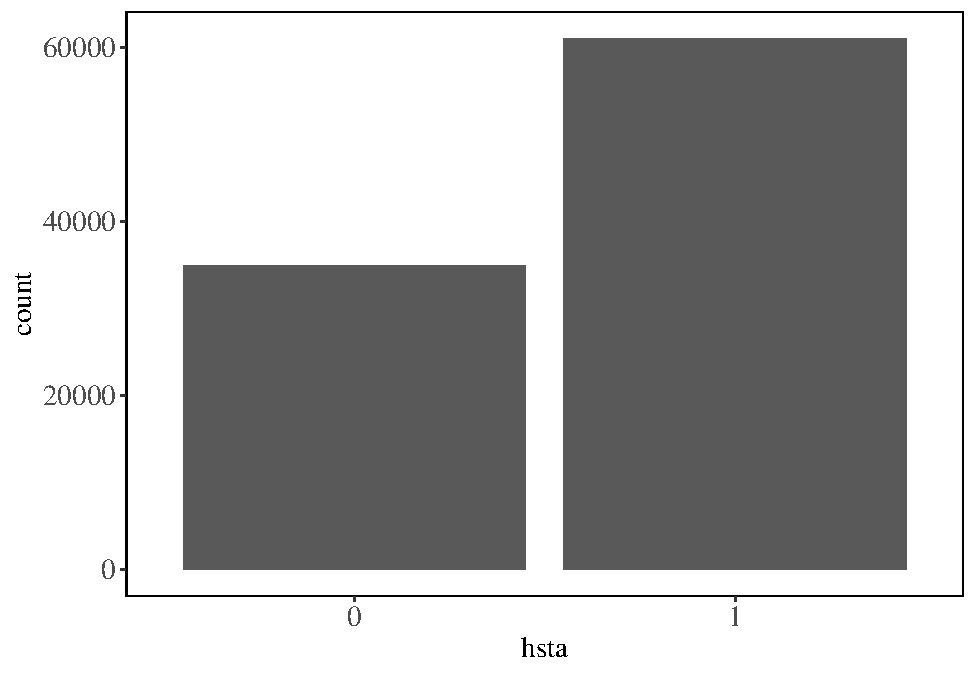
\includegraphics{Simplify_files/figure-latex/unnamed-chunk-1-1.pdf}

Það lítur út fyrir að vera mikið meira af gögnunum sem eru svör sem hafa sést áður á móti nýjum svörum.
Þar sem u.þ.b. 2/3 af gögnunum eru spurningar með rétt svör sem hafa sést áður á meðan 1/3 af gögnunum eru spurningar með rétt svör sem eru að sjást í fyrsta sinn.

Nú markmiðið er að geta skoðað framfarir nemenda, ekki bara utanaðbókarlærdóm, svo það væri gott að setja upp graf sem inniheldur meðaltal réttra svara fyrir hvert fsfa og skipt eftir hsta. Semsagt meðaltal réttra svara hjá þeim sem hafa séð x margar spurningar hingað til, bæði fyrir þann fjölda sem hefur séð rétta svarið áður og þau sem hafa það ekki.

\begin{figure}
\centering
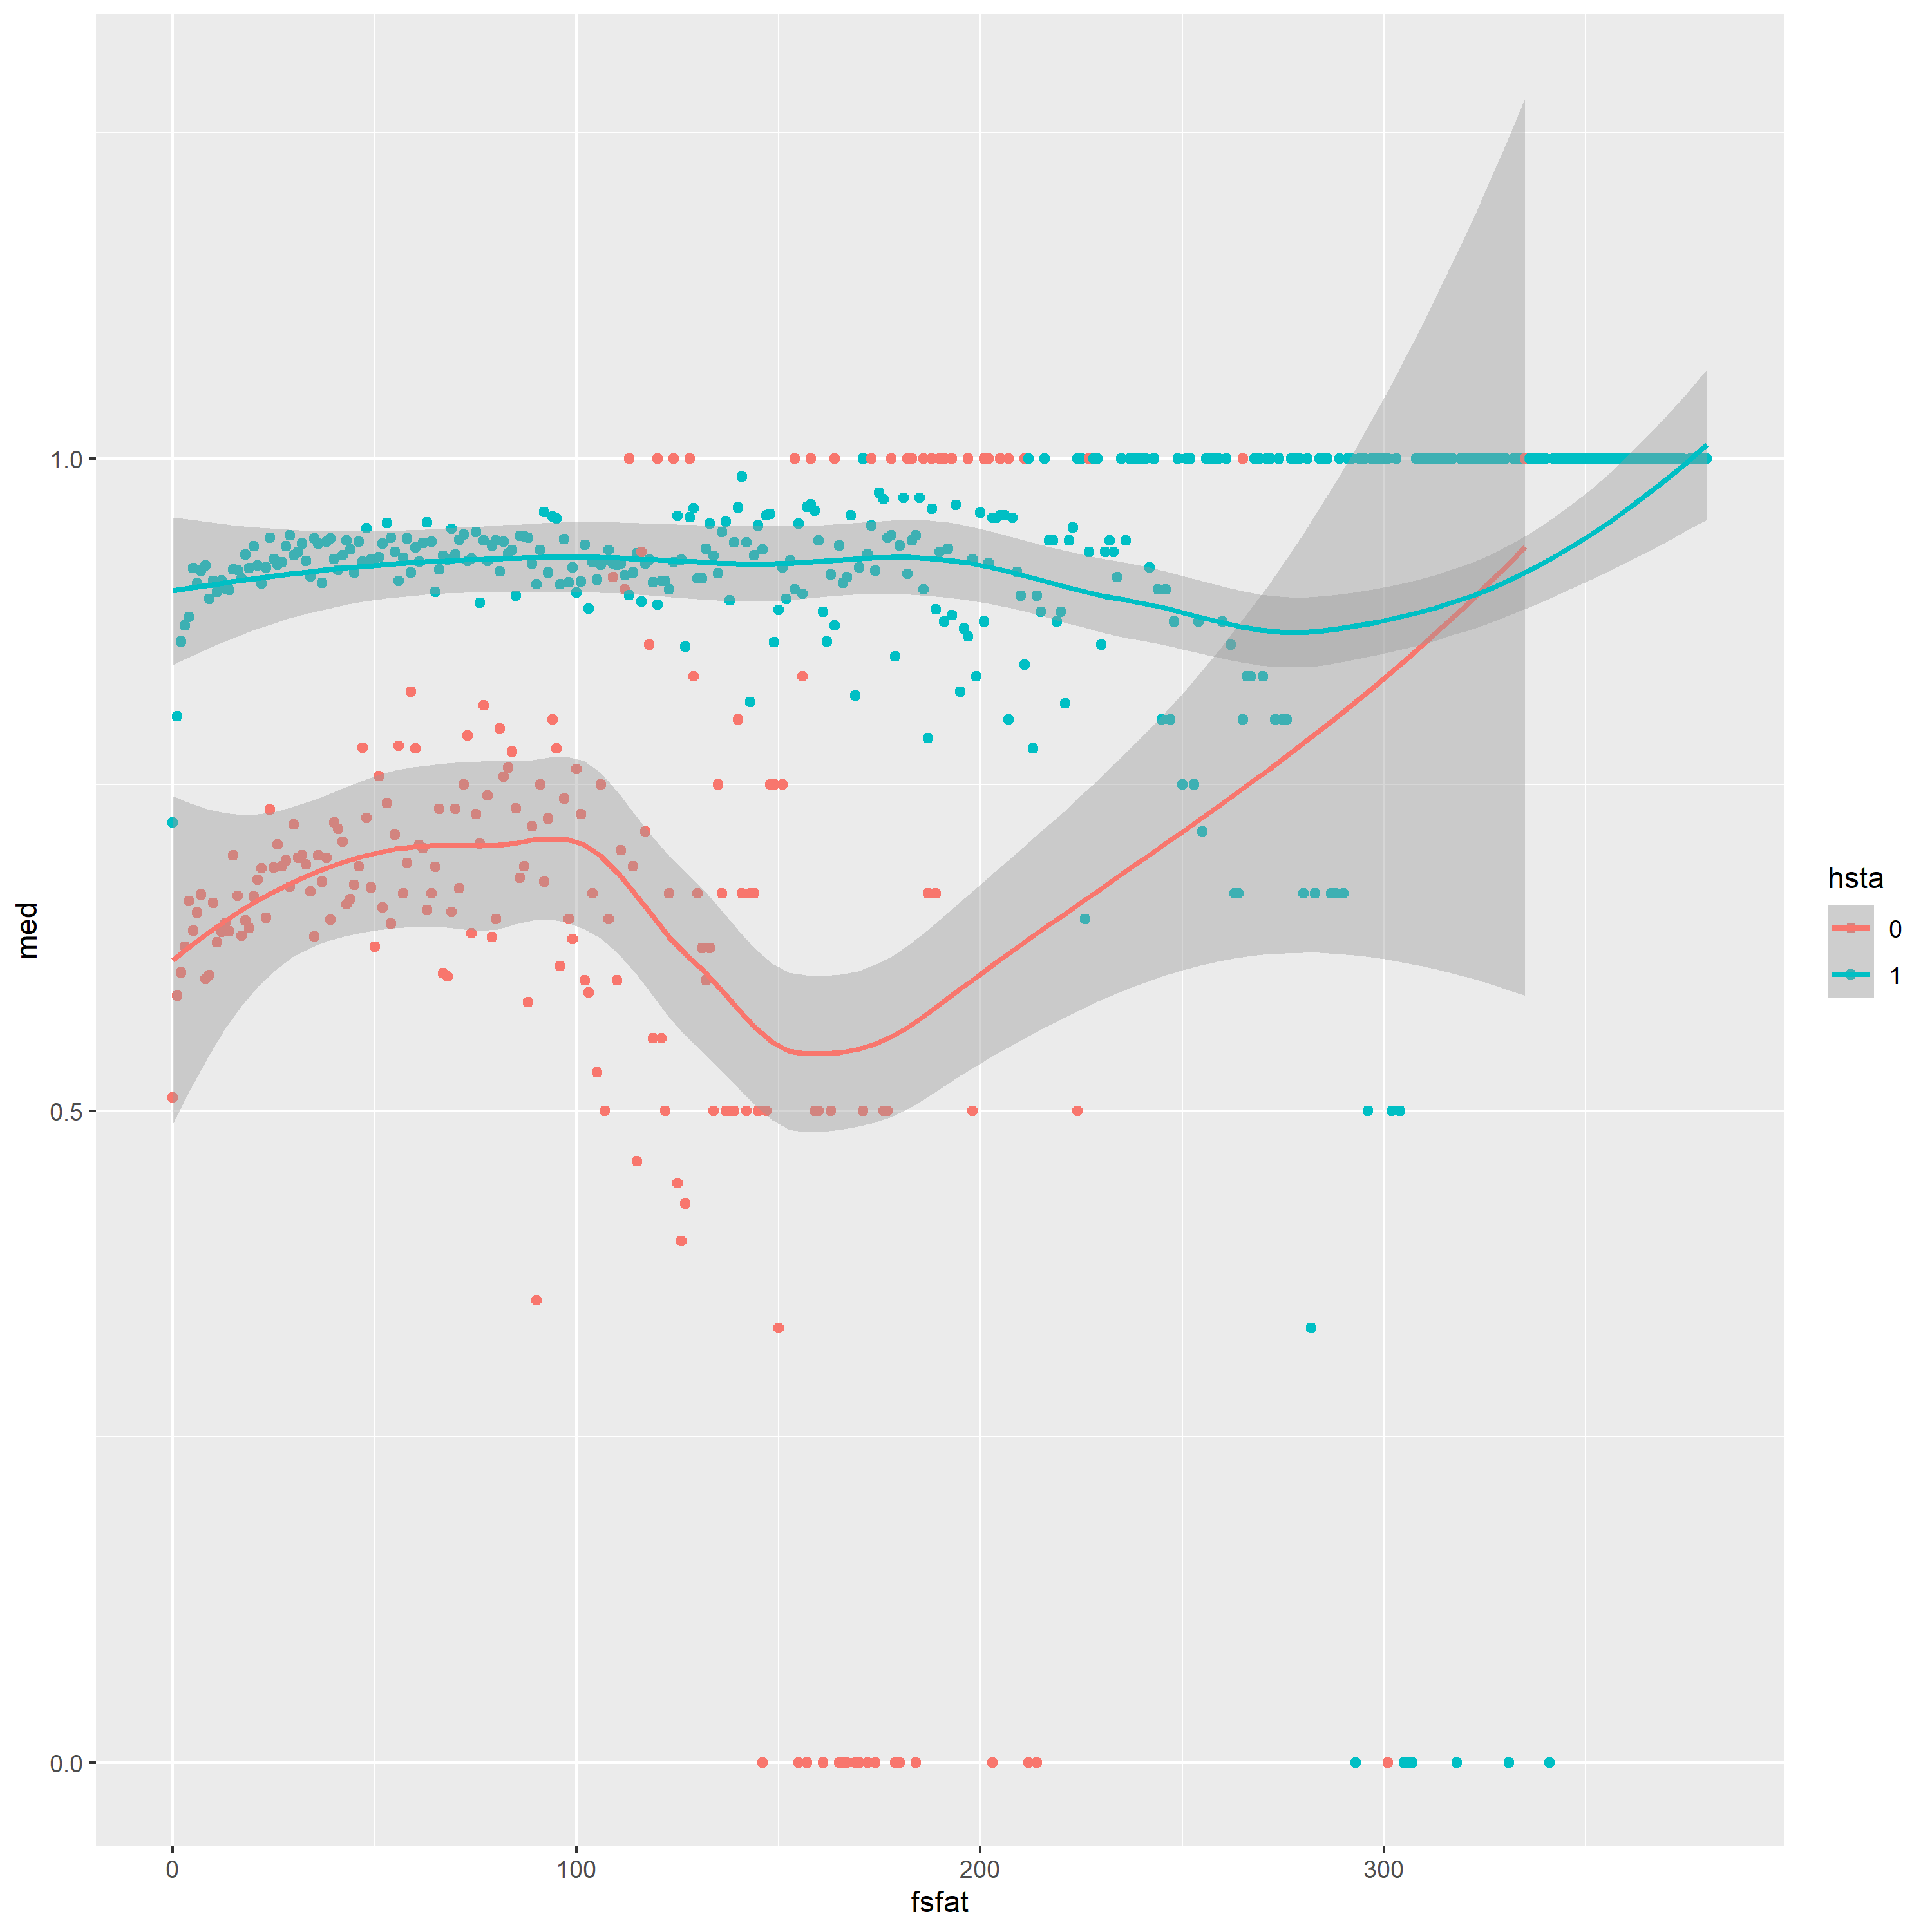
\includegraphics{Imgsimplify/plotbymean.png}
\caption{plot by mean}
\end{figure}

Það er nú smá erfitt að lesa þessa mynd, það lítur út fyrir að vera smá vaxi hjá þeim sem eru að sjá þetta í fyrsta skiptið, svo fellur það niður og aftur upp. Svo er dreifnin að vaxa því lengra sem er farið. Skoðum aðeins stærð gagnanna fyrir hvern punkt til að sjá hvað er að gerast

\begin{figure}
\centering
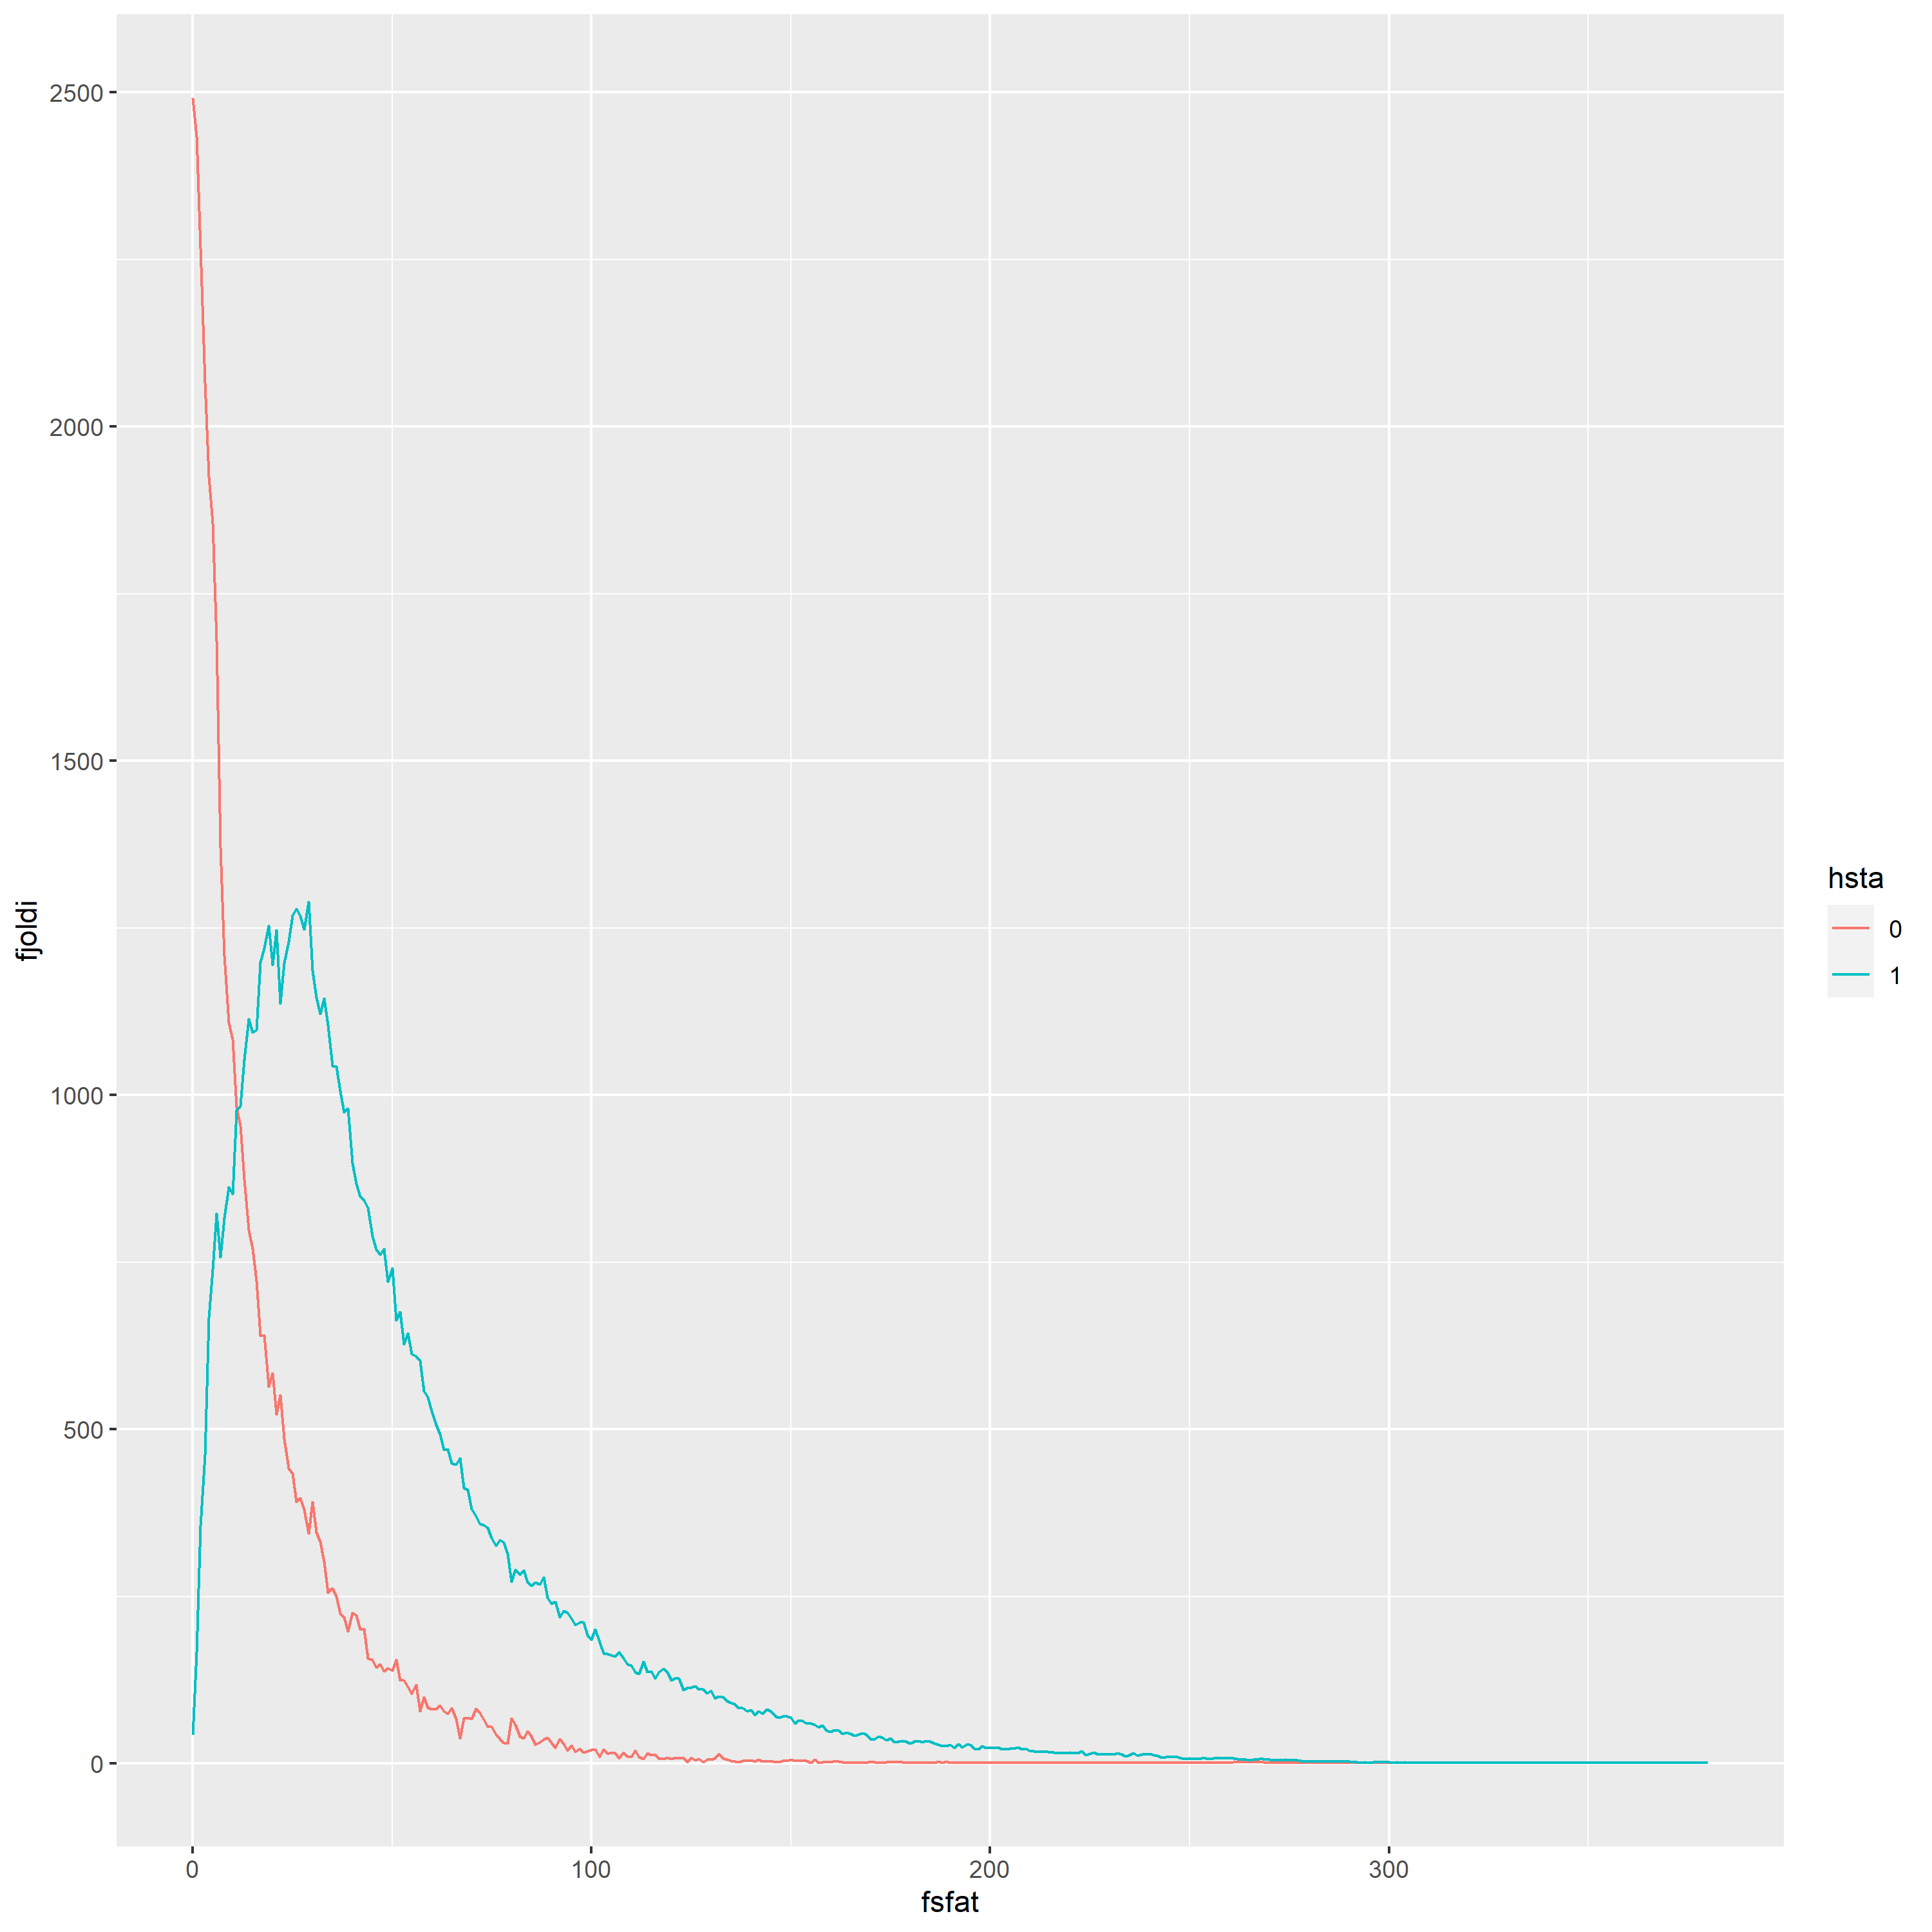
\includegraphics{Imgsimplify/plotbyamount.png}
\caption{plot by sum}
\end{figure}

Hérna kemur skýringinn, það lítur út fyrir að vera stórt fall af gögnum sem eru að sjá svar í fyrsta sinn því lengra sem er farið, og líka hjá þeim sem hafa séð svarið áður. Þetta er líklega útaf því að hver nemandi fer mismunandi langt og sumir nemendur geta verið að fara lengur en hinir. Skoðum aðeins hlutföll gagnanna til að skoða þetta betur.

\begin{Shaded}
\begin{Highlighting}[]
\NormalTok{a <-}\StringTok{ }\NormalTok{hashAnswer }\OperatorTok\StringTok{ }\KeywordTok{summarise}\NormalTok{(}\StringTok{"FY50"}\NormalTok{ =}\StringTok{ }\KeywordTok{sum}\NormalTok{(fsfat }\OperatorTok{>=}\StringTok{ }\DecValTok{50}\NormalTok{), }\StringTok{"FY100"}\NormalTok{ =}\StringTok{ }\KeywordTok{sum}\NormalTok{(fsfat }\OperatorTok{>=}\StringTok{ }\DecValTok{100}\NormalTok{), }
                              \StringTok{"FY150"}\NormalTok{ =}\StringTok{ }\KeywordTok{sum}\NormalTok{(fsfat }\OperatorTok{>=}\StringTok{ }\DecValTok{150}\NormalTok{), }\StringTok{"FY200"}\NormalTok{ =}\StringTok{ }\KeywordTok{sum}\NormalTok{(fsfat }\OperatorTok{>=}\StringTok{ }\DecValTok{200}\NormalTok{), }
                              \StringTok{"FY250"}\NormalTok{ =}\StringTok{ }\KeywordTok{sum}\NormalTok{(fsfat }\OperatorTok{>=}\StringTok{ }\DecValTok{250}\NormalTok{), }\StringTok{"FY300"}\NormalTok{ =}\StringTok{ }\KeywordTok{sum}\NormalTok{(fsfat }\OperatorTok{>=}\StringTok{ }\DecValTok{300}\NormalTok{))}
\NormalTok{b <-}\StringTok{ }\NormalTok{hashAnswer }\OperatorTok\StringTok{ }\KeywordTok{summarise}\NormalTok{(}\StringTok{"HY50"}\NormalTok{ =}\StringTok{ }\KeywordTok{mean}\NormalTok{(fsfat }\OperatorTok{>=}\StringTok{ }\DecValTok{50}\NormalTok{), }\StringTok{"HY100"}\NormalTok{ =}\StringTok{ }\KeywordTok{mean}\NormalTok{(fsfat }\OperatorTok{>=}\StringTok{ }\DecValTok{100}\NormalTok{), }
                              \StringTok{"HY150"}\NormalTok{ =}\StringTok{ }\KeywordTok{mean}\NormalTok{(fsfat }\OperatorTok{>=}\StringTok{ }\DecValTok{150}\NormalTok{), }\StringTok{"HY200"}\NormalTok{ =}\StringTok{ }\KeywordTok{mean}\NormalTok{(fsfat }\OperatorTok{>=}\StringTok{ }\DecValTok{200}\NormalTok{), }
                              \StringTok{"HY250"}\NormalTok{ =}\StringTok{ }\KeywordTok{mean}\NormalTok{(fsfat }\OperatorTok{>=}\StringTok{ }\DecValTok{250}\NormalTok{), }\StringTok{"HY300"}\NormalTok{ =}\StringTok{ }\KeywordTok{mean}\NormalTok{(fsfat }\OperatorTok{>=}\StringTok{ }\DecValTok{300}\NormalTok{))}
\NormalTok{ab <-}\StringTok{ }\KeywordTok{cbind}\NormalTok{(a, b)}
\NormalTok{FHbylim <-}\StringTok{ }\NormalTok{ab }\OperatorTok\StringTok{ }\KeywordTok{pivot_longer}\NormalTok{(}\KeywordTok{c}\NormalTok{(}\StringTok{'FY50'}\NormalTok{, }\StringTok{'HY50'}\NormalTok{, }\StringTok{'FY100'}\NormalTok{, }\StringTok{'HY100'}\NormalTok{, }\StringTok{'FY150'}\NormalTok{, }\StringTok{'HY150'}\NormalTok{, }\StringTok{'FY200'}\NormalTok{, }\StringTok{'HY200'}\NormalTok{, }\StringTok{'FY250'}\NormalTok{, }\StringTok{'HY250'}\NormalTok{, }\StringTok{'FY300'}\NormalTok{, }\StringTok{'HY300'}\NormalTok{), }
                    \DataTypeTok{names_to =} \StringTok{"typewLim"}\NormalTok{, }\DataTypeTok{values_to =} \StringTok{"values"}\NormalTok{) }\OperatorTok\StringTok{ }
\StringTok{  }\KeywordTok{separate}\NormalTok{(typewLim, }\DataTypeTok{into =} \KeywordTok{c}\NormalTok{(}\StringTok{"type"}\NormalTok{, }\StringTok{"limit"}\NormalTok{), }\DataTypeTok{sep =} \DecValTok{2}\NormalTok{) }\OperatorTok\StringTok{ }\KeywordTok{pivot_wider}\NormalTok{(}\DataTypeTok{names_from =}\NormalTok{ type, }\DataTypeTok{values_from =}\NormalTok{ values)}


\NormalTok{FHbylim }\OperatorTok\StringTok{ }\KeywordTok{kable}\NormalTok{(}\DataTypeTok{digits =} \DecValTok{4}\NormalTok{)}
\end{Highlighting}
\end{Shaded}

\begin{tabular}{l|r|r}
\hline
limit & FY & HY\\
\hline
50 & 28325 & 0.2950\\
\hline
100 & 8734 & 0.0910\\
\hline
150 & 2970 & 0.0309\\
\hline
200 & 1098 & 0.0114\\
\hline
250 & 323 & 0.0034\\
\hline
300 & 84 & 0.0009\\
\hline
\end{tabular}

Lítur út fyrir að um 27.75\% gagnanna eru af spurningum sem fara yfir 50 fsfat og bara u.þ.b. 8.29\% gagnanna sem fara yfir 100. Hugmynd er þá að skera af gögninn miðað við 50 fsfat eða 100 fsfat. Skoðum þá aðeins hlutfall hsta og meðtalals grafið að ofan miðað við það.

\hypertarget{skouxf0auxf0-eftir-limit}{%
\subsection{Skoðað eftir limit}\label{skouxf0auxf0-eftir-limit}}

Fyrst er að setja upp gögninn. Að auki fjarlægji ég nemendur sem svöruðu ekki fleiri en 7 spurningum samtals

\begin{Shaded}
\begin{Highlighting}[]
\NormalTok{hashLim50 <-}\StringTok{ }\NormalTok{hashAnswer }\OperatorTok\StringTok{ }\KeywordTok{group_by}\NormalTok{(studentId) }\OperatorTok\StringTok{ }\KeywordTok{mutate}\NormalTok{(}\StringTok{"count"}\NormalTok{ =}\StringTok{ }\KeywordTok{n}\NormalTok{()) }\OperatorTok
\StringTok{  }\KeywordTok{filter}\NormalTok{(count }\OperatorTok{>}\StringTok{ }\DecValTok{7} \OperatorTok{&}\StringTok{ }\NormalTok{fsfat }\OperatorTok{<}\StringTok{ }\DecValTok{50}\NormalTok{)}
\NormalTok{hashLim100 <-}\StringTok{ }\NormalTok{hashAnswer }\OperatorTok\StringTok{ }\KeywordTok{group_by}\NormalTok{(studentId) }\OperatorTok\StringTok{ }\KeywordTok{mutate}\NormalTok{(}\StringTok{"count"}\NormalTok{ =}\StringTok{ }\KeywordTok{n}\NormalTok{()) }\OperatorTok
\StringTok{  }\KeywordTok{filter}\NormalTok{(count }\OperatorTok{>}\StringTok{ }\DecValTok{7} \OperatorTok{&}\StringTok{ }\NormalTok{fsfat }\OperatorTok{<}\StringTok{ }\DecValTok{100}\NormalTok{)}
\end{Highlighting}
\end{Shaded}

Skoðum hlutfallið aftur hjá hsta.

\begin{Shaded}
\begin{Highlighting}[]
\KeywordTok{ggplot}\NormalTok{(hashLim50, }\KeywordTok{aes}\NormalTok{(}\DataTypeTok{x =}\NormalTok{ hsta)) }\OperatorTok{+}
\StringTok{  }\KeywordTok{geom_bar}\NormalTok{() }\OperatorTok{+}\StringTok{ }
\StringTok{  }\KeywordTok{ggtitle}\NormalTok{(}\StringTok{"undir 50"}\NormalTok{)}
\end{Highlighting}
\end{Shaded}

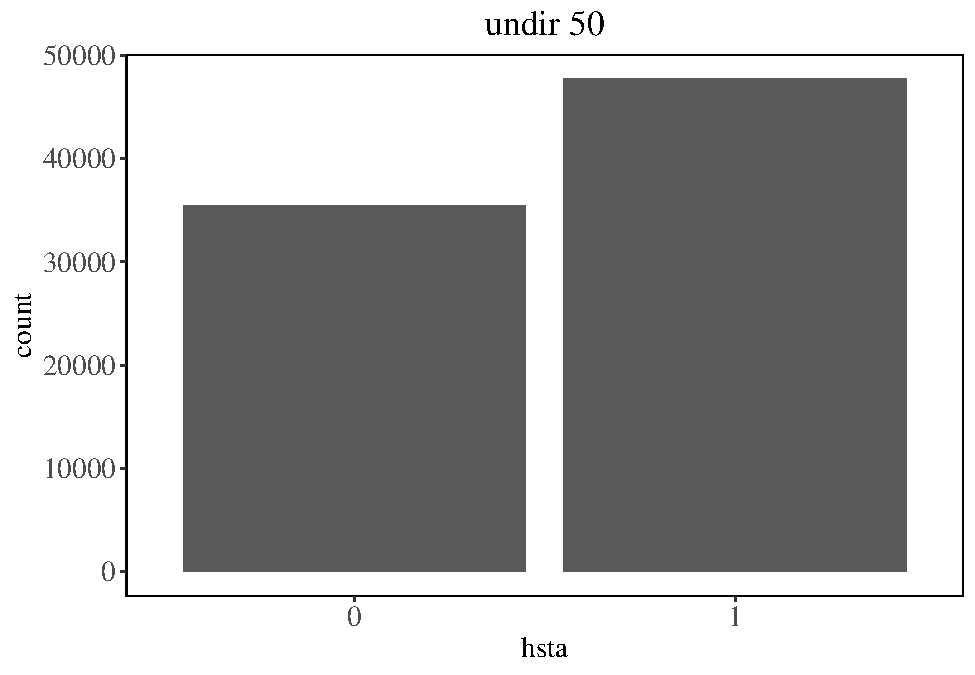
\includegraphics{Simplify_files/figure-latex/unnamed-chunk-3-1.pdf}

\begin{Shaded}
\begin{Highlighting}[]
\KeywordTok{ggplot}\NormalTok{(hashLim100, }\KeywordTok{aes}\NormalTok{(}\DataTypeTok{x =}\NormalTok{ hsta)) }\OperatorTok{+}
\StringTok{  }\KeywordTok{geom_bar}\NormalTok{() }\OperatorTok{+}\StringTok{ }
\StringTok{  }\KeywordTok{ggtitle}\NormalTok{(}\StringTok{"undir 100"}\NormalTok{)}
\end{Highlighting}
\end{Shaded}

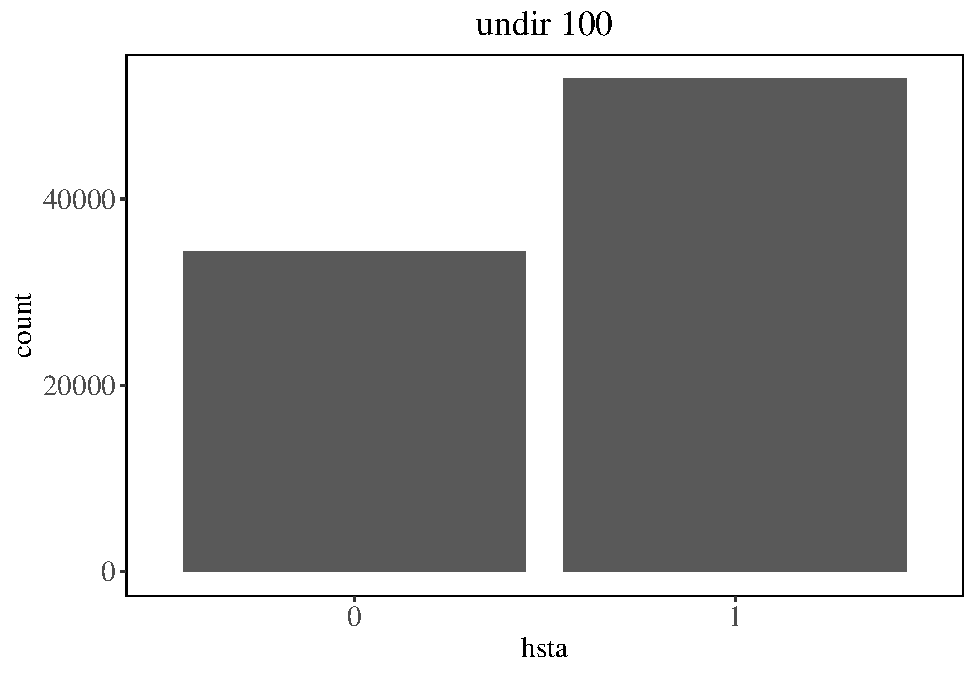
\includegraphics{Simplify_files/figure-latex/unnamed-chunk-3-2.pdf}

Það sést að ef við tökum bara undir 50, þá er hsta orðið miklu nær og þegar við erum með undir 100, þá erum við kominn nálægt ójöfnunni eins og áðan.

Gott að skoða meðaltals myndina aftur, eftir að skera eftir limit.

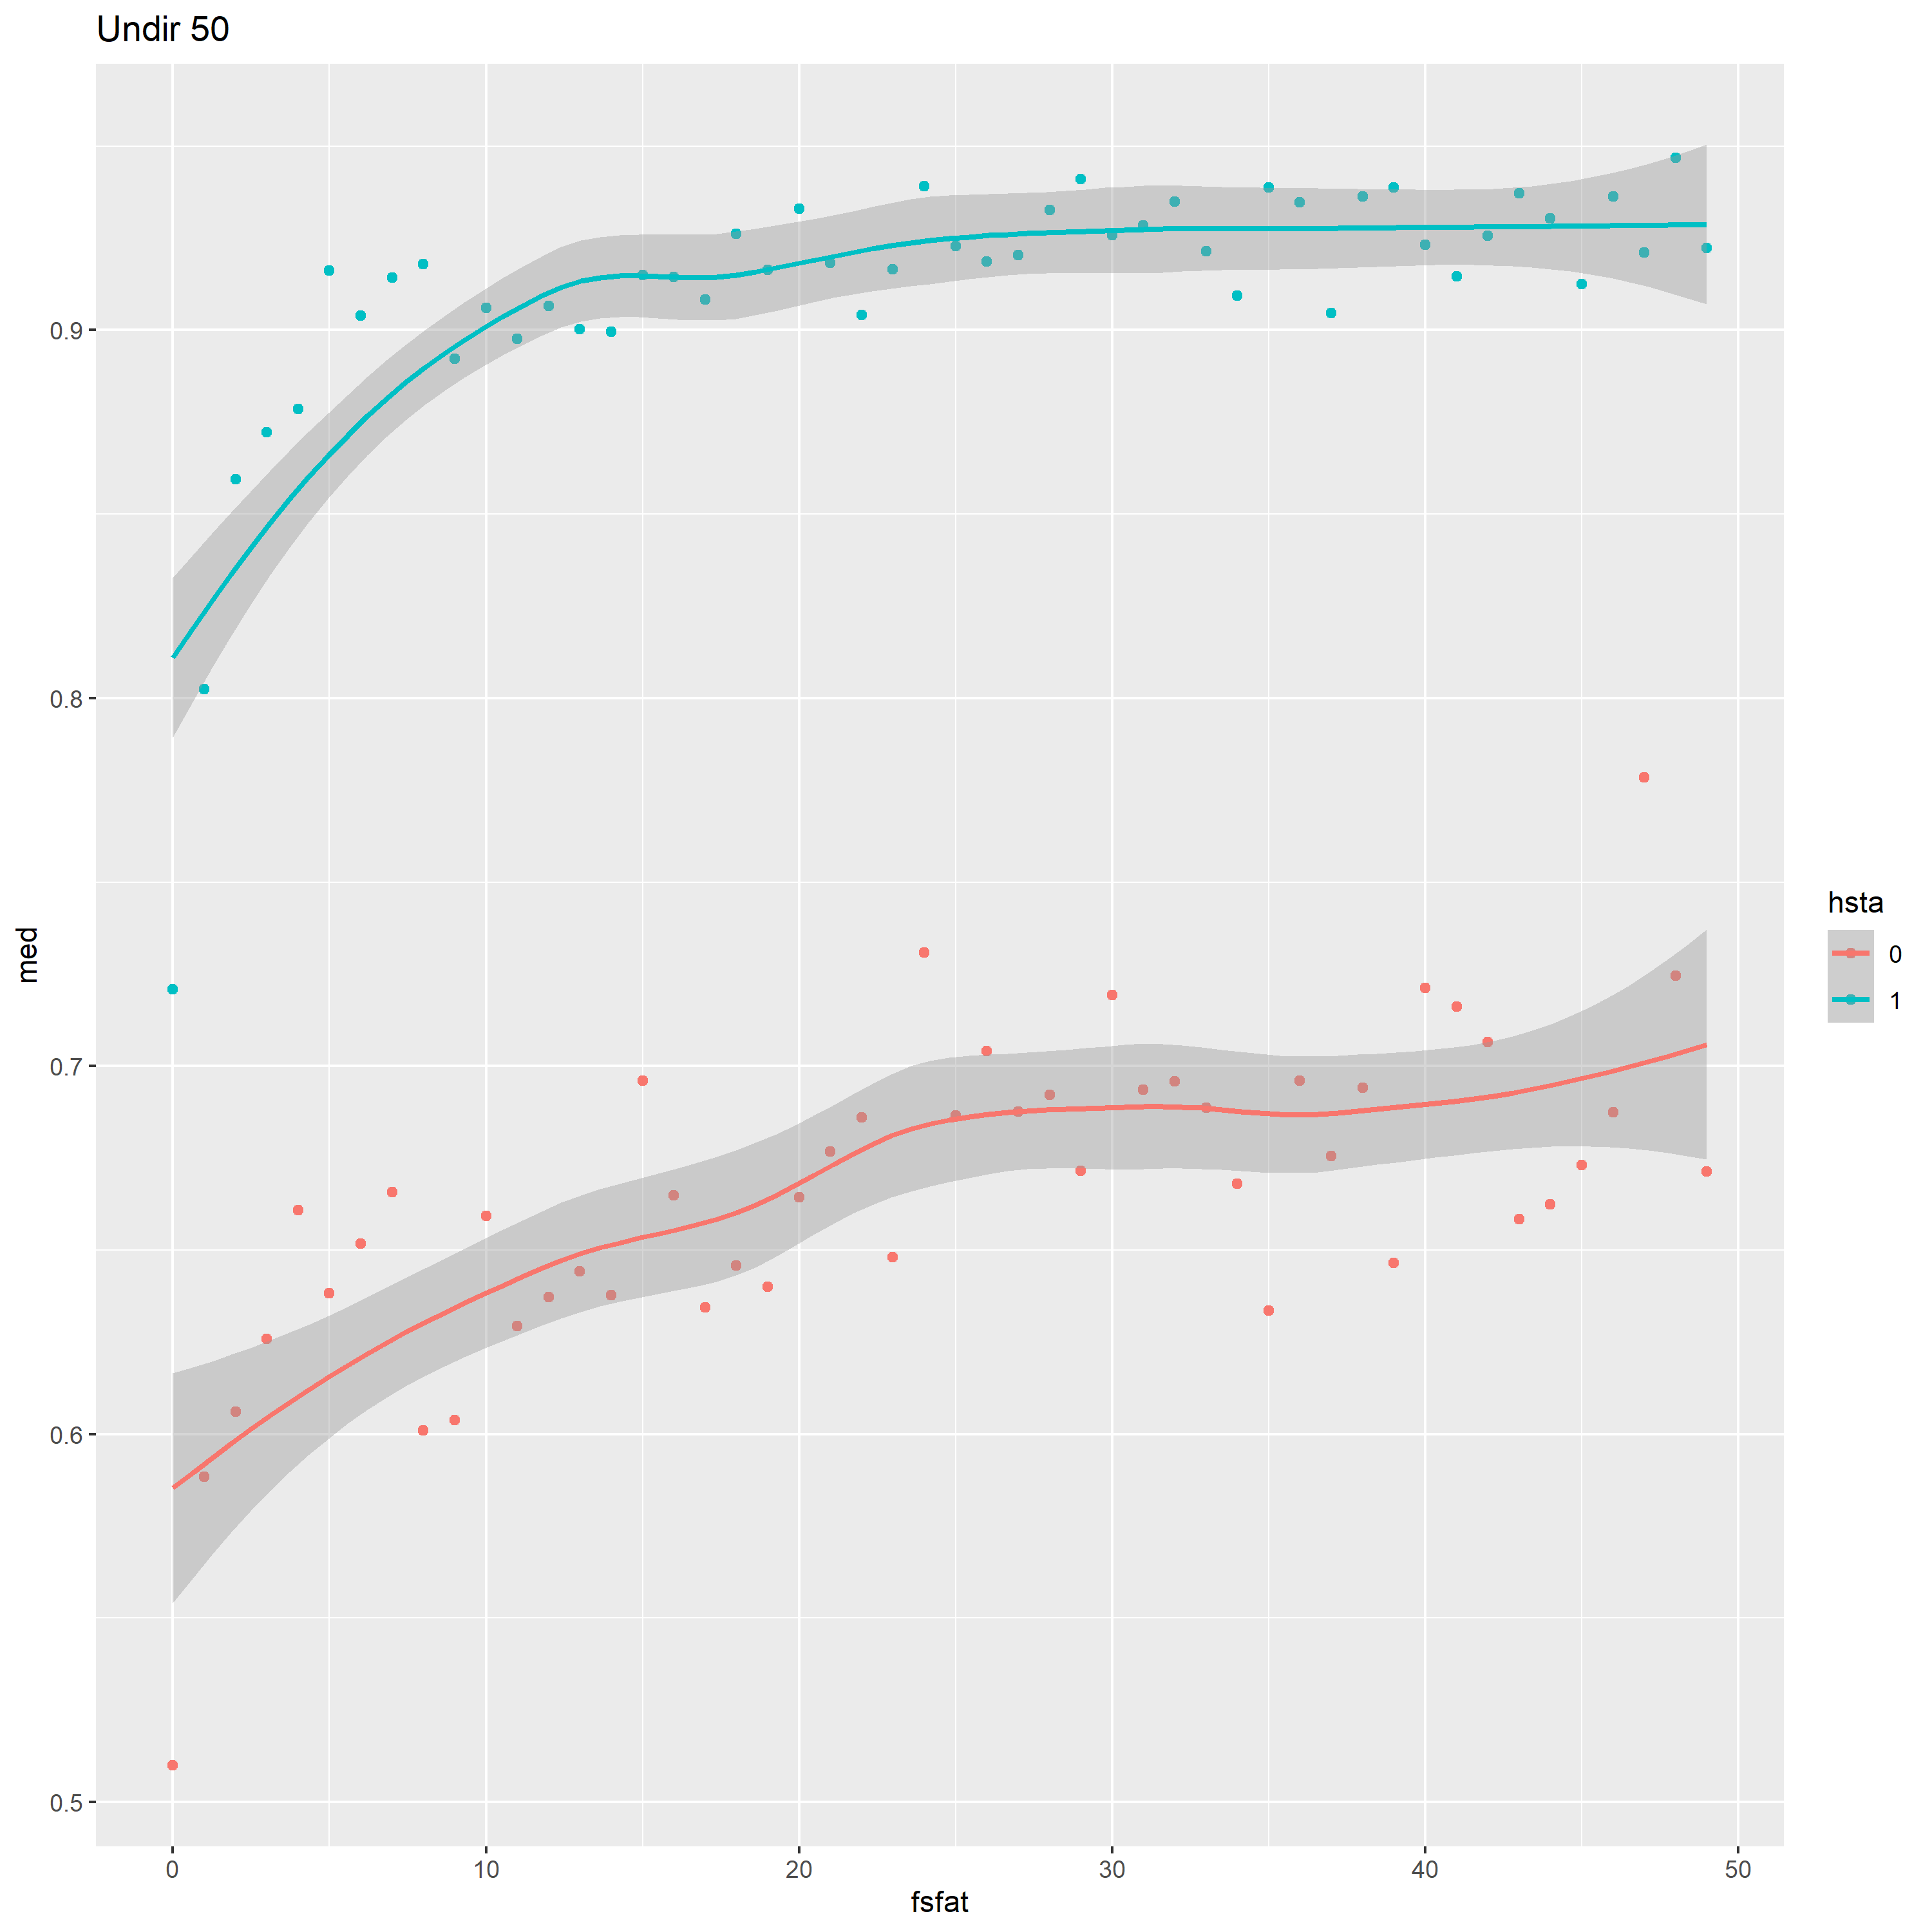
\includegraphics{Imgsimplify/plotbymean50.png}
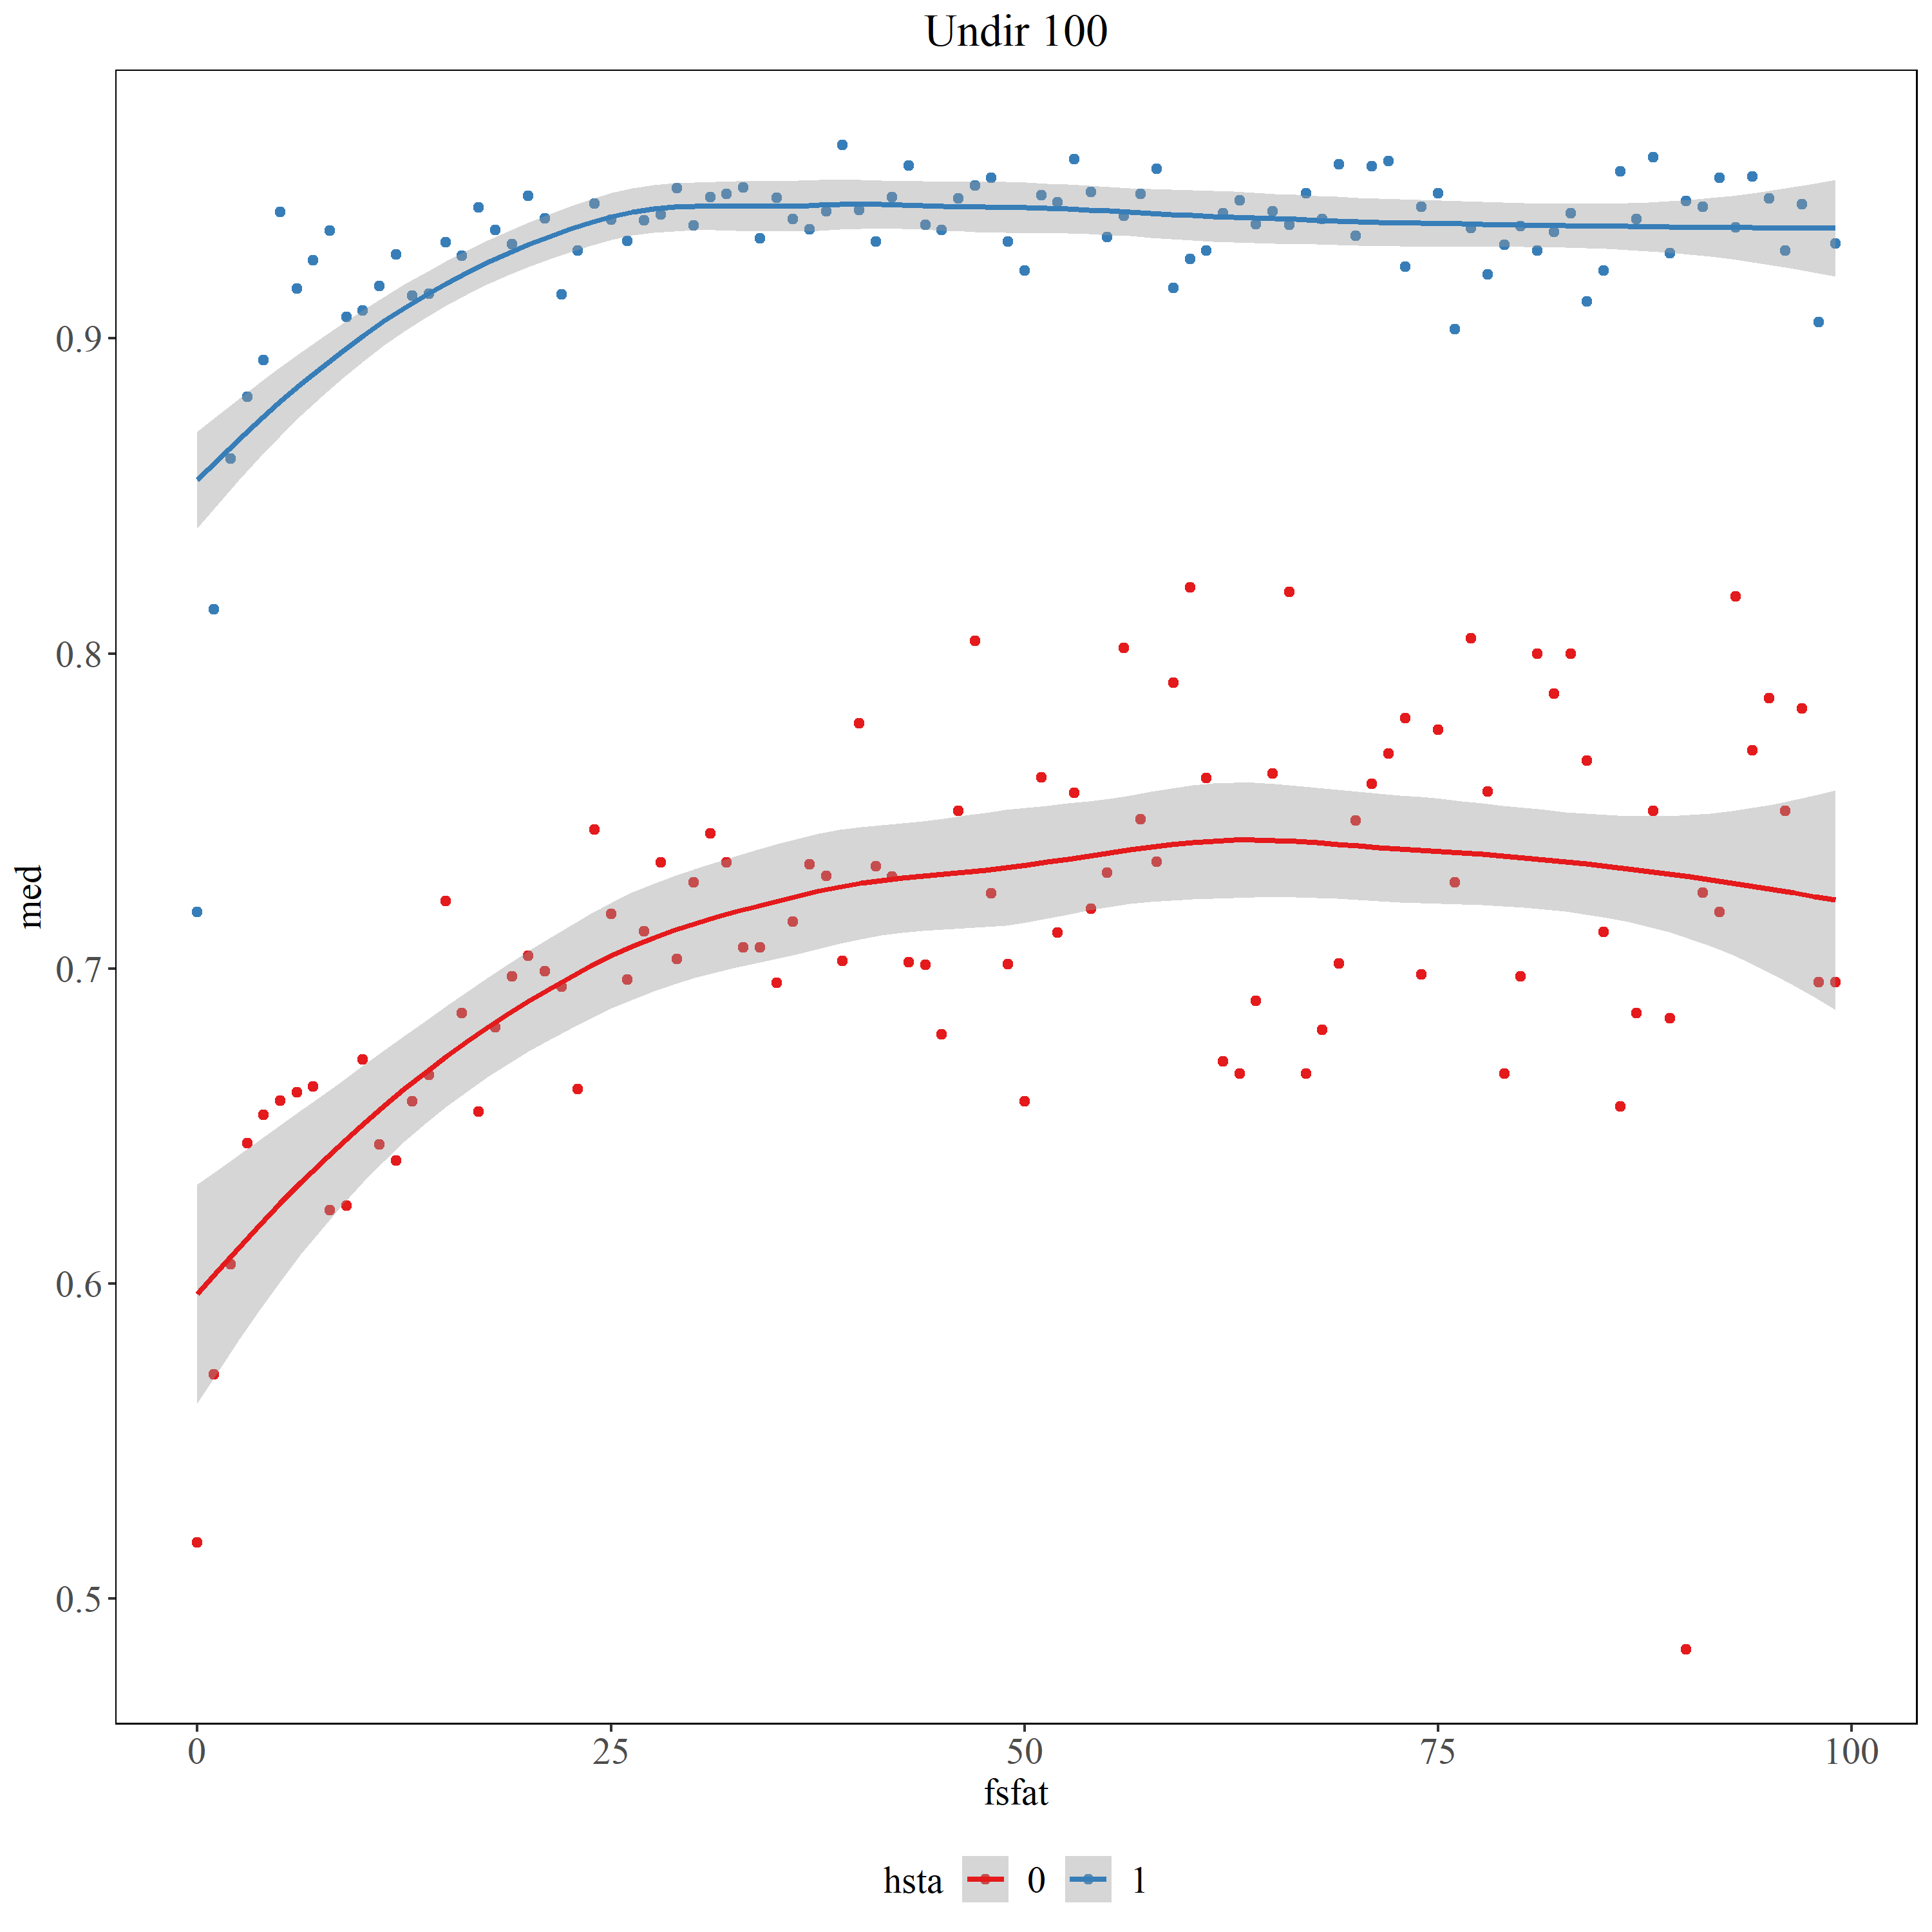
\includegraphics{Imgsimplify/plotbymean100.png}

Nú sést aðeins betur hvað er að gerast, í fyrri sjáum við að það lítur út fyrir að vera árangur og framfarir. Þar sem báðar línunar eru að vaxa þegar fleiri spurninga hefur verið svarað. En það sést á seinni myndini að það fer að jafna sig eftir það og framfarir hætta. Svo er það eitthvað smá fall hjá nýjum svörum.

\hypertarget{umruxe6uxf0ur}{%
\subsection{umræður}\label{umruxe6uxf0ur}}

Þá kemur spurninginn hvort þetta er nokkuð framfarir eða utanaðbókarlærdómur, í fyrri þá lítur út fyrir að líkurnar vaxa. En það virðist svo jafna sig eftir það.

\begin{enumerate}
\def\labelenumi{\arabic{enumi}.}
\tightlist
\item
  Ein hugmynd um hvað er að gerast þar er að þetta er ekki framfarir sem er að vaxa, heldur er það utanaðbókarlærdómur á röngu svarmöguleikunum, Það gæti verið aðal áhrifinn þar. Hugmynd til að skoða það betur væri kannski að skoða eins mynd, nema filterað bara fyrir spurningarnar sem hafa rétt svör sem eru að sjást í fyrsta skiptið og gert flokka fyrir hlutfall rangra svara sem hafa sést áður. Þá mun koma ein lína fyrir hvert hlutfall, ef það er allt beinar láréttar línur, þá gæti það bent til að verið sé að ræða utanaðbókarlærdómur sem aðal áhrifin.
\item
  Önnur hugmynd er að ef við gætum skipt nemendum upp í flokka, sem nemendur sem setja allt á minnið og nemendur sem eru að læra og fá framfarir. Svo er spurning hvort framfarirnar sjást betur þa.
\item
  Loka hugmynd er að í staðinn fyrir að skoða fsfat eftir fyrirlestri, að skoða það kannski frekar eftir spurningahaus, þá gæti sést betur áhrif á sambærilegum spurningum eftir því hve margar tilraunir nemandinn hefur fengið á spurninguna sjálfa.
\end{enumerate}

\hypertarget{modelgeruxf0}{%
\section{Modelgerð}\label{modelgeruxf0}}

Hér er smá grunnur af því sem ég er kominn með fyrir modelgerðina.

Ég byrjaði að skoða einföld glm, en þar sem það er verið að ræða um mixed effect model, þá hef ég fært yfir í glmer í staðinn. Ég ákvað að keyra allt miðað við 100 limitinn, ég hef ekki neina sterka ástæðu enn, þar sem ég veit ekki um leið til að sýna hvort einn gagnasett er betri en hitt, svo mér fannst 100 vera nægilega gott í bili.

\hypertarget{gagnavinnsla}{%
\subsection{gagnavinnsla}\label{gagnavinnsla}}

Fyrsta sem þarf að gera, er smá gagnavinnsla. Glmer tekur ekki vel við háu tölunum í fsfat, svo ég deili með 10 til að fá glmer til að keyra almennilega

\begin{Shaded}
\begin{Highlighting}[]
\NormalTok{hashLim100}\OperatorTok{$}\NormalTok{fsfat <-}\StringTok{ }\NormalTok{hashLim100}\OperatorTok{$}\NormalTok{fsfat}\OperatorTok{/}\DecValTok{10}
\end{Highlighting}
\end{Shaded}

\hypertarget{modelin-sjuxe1lf}{%
\subsection{modelin sjálf}\label{modelin-sjuxe1lf}}

Modelinn sem ég er að vinna með á þessum tímapunkti er

\begin{itemize}
\item
  glmer(correct \textasciitilde{} fsfat*hsta + nicc + gpow + lectureId + (1 \textbar{} studentId), family = binomial(link = ``logit''), \ldots)
\item
  glmer(correct \textasciitilde{} fsfat*hsta + nicc + gpow + lectureId + (1 + fsfat * hsta \textbar{} studentId), family = binomial(link = ``logit''), \ldots)
\end{itemize}

Stóri munurinn milli þeirra er að ég hef meira í mixed effect modelinu seinna en í því fyrra

Ég keyri módelinn ekki hér, því þau eru of löng, en hef save-að þau til seinni notkunar, svo hægt sé að load-a þeim upp

\begin{Shaded}
\begin{Highlighting}[]
\CommentTok{# #Þetta er fyrri modelið}
\CommentTok{# load("Data/ans22")}
\CommentTok{# #Þetta er seinna modelið}
\CommentTok{# load("Data/ans42")}
\end{Highlighting}
\end{Shaded}

\hypertarget{uppfuxe6rt-auxf0feruxf0-til-auxf0-keyra-hrauxf0ar}{%
\subsubsection{Uppfært aðferð til að keyra hraðar}\label{uppfuxe6rt-auxf0feruxf0-til-auxf0-keyra-hrauxf0ar}}

\begin{Shaded}
\begin{Highlighting}[]
\KeywordTok{options}\NormalTok{(}\DataTypeTok{contrasts =} \KeywordTok{c}\NormalTok{(}\StringTok{"contr.sum"}\NormalTok{, }\StringTok{"contr.poly"}\NormalTok{))}
\NormalTok{ans22 <-}\StringTok{ }\KeywordTok{glmer}\NormalTok{(correct }\OperatorTok{~}\StringTok{ }\NormalTok{fsfat}\OperatorTok{*}\NormalTok{hsta }\OperatorTok{+}\StringTok{ }\NormalTok{nicc }\OperatorTok{+}\StringTok{ }\NormalTok{gpow }\OperatorTok{+}\StringTok{ }\NormalTok{lectureId }\OperatorTok{+}\StringTok{ }\NormalTok{(}\DecValTok{1} \OperatorTok{|}\StringTok{ }\NormalTok{studentId), }\DataTypeTok{family =} \KeywordTok{binomial}\NormalTok{(}\DataTypeTok{link =} \StringTok{"logit"}\NormalTok{), }
               \DataTypeTok{data =}\NormalTok{ hashLim100, }\DataTypeTok{nAGQ =} \DecValTok{0}\NormalTok{, }\DataTypeTok{control=}\KeywordTok{glmerControl}\NormalTok{(}\DataTypeTok{optimizer=}\StringTok{"bobyqa"}\NormalTok{,}\DataTypeTok{optCtrl=}\KeywordTok{list}\NormalTok{(}\DataTypeTok{maxfun=}\FloatTok{2e5}\NormalTok{)))}
\NormalTok{ans42 <-}\StringTok{ }\KeywordTok{glmer}\NormalTok{(correct }\OperatorTok{~}\StringTok{ }\NormalTok{fsfat}\OperatorTok{*}\NormalTok{hsta }\OperatorTok{+}\StringTok{ }\NormalTok{nicc }\OperatorTok{+}\StringTok{ }\NormalTok{gpow }\OperatorTok{+}\StringTok{ }\NormalTok{lectureId }\OperatorTok{+}\StringTok{ }\NormalTok{(}\DecValTok{1} \OperatorTok{+}\StringTok{ }\NormalTok{fsfat }\OperatorTok{*}\StringTok{ }\NormalTok{hsta }\OperatorTok{|}\StringTok{ }\NormalTok{studentId), }
               \DataTypeTok{family =} \KeywordTok{binomial}\NormalTok{(}\DataTypeTok{link =} \StringTok{"logit"}\NormalTok{), }\DataTypeTok{data =}\NormalTok{ hashLim100, }\DataTypeTok{nAGQ =} \DecValTok{0}\NormalTok{,}
               \DataTypeTok{control=}\KeywordTok{glmerControl}\NormalTok{(}\DataTypeTok{optimizer=}\StringTok{"bobyqa"}\NormalTok{,}\DataTypeTok{optCtrl=}\KeywordTok{list}\NormalTok{(}\DataTypeTok{maxfun=}\FloatTok{2e5}\NormalTok{)))}
\end{Highlighting}
\end{Shaded}

\hypertarget{smuxe1-model-analysis}{%
\subsection{smá model Analysis}\label{smuxe1-model-analysis}}

Summaríið þeirra er svo

\begin{Shaded}
\begin{Highlighting}[]
\KeywordTok{summary}\NormalTok{(ans22)}
\end{Highlighting}
\end{Shaded}

\begin{verbatim}
## Generalized linear mixed model fit by maximum likelihood (Adaptive
##   Gauss-Hermite Quadrature, nAGQ = 0) [glmerMod]
##  Family: binomial  ( logit )
## Formula: correct ~ fsfat * hsta + nicc + gpow + lectureId + (1 | studentId)
##    Data: hashLim100
## Control: glmerControl(optimizer = "bobyqa", optCtrl = list(maxfun = 2e+05))
## 
##      AIC      BIC   logLik deviance df.resid 
##  62028.4  62253.4 -30990.2  61980.4    87232 
## 
## Scaled residuals: 
##      Min       1Q   Median       3Q      Max 
## -11.9180   0.1437   0.2316   0.4062   3.7665 
## 
## Random effects:
##  Groups    Name        Variance Std.Dev.
##  studentId (Intercept) 0.7562   0.8696  
## Number of obs: 87256, groups:  studentId, 283
## 
## Fixed effects:
##              Estimate Std. Error z value Pr(>|z|)    
## (Intercept)  1.659542   0.062155  26.700  < 2e-16 ***
## fsfat        0.203916   0.005618  36.297  < 2e-16 ***
## hsta1       -1.069679   0.019517 -54.808  < 2e-16 ***
## nicc1        0.611590   0.136589   4.478 7.55e-06 ***
## nicc2        0.309886   0.054664   5.669 1.44e-08 ***
## nicc3       -0.140135   0.029050  -4.824 1.41e-06 ***
## nicc4       -0.032914   0.037133  -0.886 0.375404    
## nicc5       -0.211427   0.035790  -5.907 3.47e-09 ***
## nicc6       -0.273325   0.035506  -7.698 1.38e-14 ***
## gpow         0.127291   0.035618   3.574 0.000352 ***
## lectureId1  -1.067109   0.027788 -38.401  < 2e-16 ***
## lectureId2   0.093693   0.038362   2.442 0.014593 *  
## lectureId3   0.615713   0.049407  12.462  < 2e-16 ***
## lectureId4  -0.582781   0.030428 -19.153  < 2e-16 ***
## lectureId5  -0.206038   0.033502  -6.150 7.75e-10 ***
## lectureId6   0.107225   0.038847   2.760 0.005777 ** 
## lectureId7   0.266837   0.042952   6.212 5.22e-10 ***
## lectureId8   0.452446   0.051391   8.804  < 2e-16 ***
## lectureId9   0.333222   0.051628   6.454 1.09e-10 ***
## lectureId10 -0.116136   0.041688  -2.786 0.005339 ** 
## lectureId11  0.076908   0.044417   1.732 0.083359 .  
## lectureId12  0.154198   0.044362   3.476 0.000509 ***
## fsfat:hsta1  0.046067   0.005156   8.935  < 2e-16 ***
## ---
## Signif. codes:  0 '***' 0.001 '**' 0.01 '*' 0.05 '.' 0.1 ' ' 1
\end{verbatim}

\begin{verbatim}
## 
## Correlation matrix not shown by default, as p = 23 > 12.
## Use print(x, correlation=TRUE)  or
##     vcov(x)        if you need it
\end{verbatim}

\begin{Shaded}
\begin{Highlighting}[]
\KeywordTok{summary}\NormalTok{(ans42)}
\end{Highlighting}
\end{Shaded}

\begin{verbatim}
## Generalized linear mixed model fit by maximum likelihood (Adaptive
##   Gauss-Hermite Quadrature, nAGQ = 0) [glmerMod]
##  Family: binomial  ( logit )
## Formula: correct ~ fsfat * hsta + nicc + gpow + lectureId + (1 + fsfat *  
##     hsta | studentId)
##    Data: hashLim100
## Control: glmerControl(optimizer = "bobyqa", optCtrl = list(maxfun = 2e+05))
## 
##      AIC      BIC   logLik deviance df.resid 
##  61585.5  61894.9 -30759.8  61519.5    87223 
## 
## Scaled residuals: 
##      Min       1Q   Median       3Q      Max 
## -12.1835   0.1301   0.2263   0.4023   3.0975 
## 
## Random effects:
##  Groups    Name        Variance Std.Dev. Corr             
##  studentId (Intercept) 0.661245 0.81317                   
##            fsfat       0.020476 0.14309   0.07            
##            hsta1       0.066818 0.25849  -0.24  0.03      
##            fsfat:hsta1 0.003598 0.05998   0.49  0.10 -0.63
## Number of obs: 87256, groups:  studentId, 283
## 
## Fixed effects:
##              Estimate Std. Error z value Pr(>|z|)    
## (Intercept)  1.571471   0.060301  26.060  < 2e-16 ***
## fsfat        0.257279   0.011425  22.520  < 2e-16 ***
## hsta1       -0.996831   0.026795 -37.202  < 2e-16 ***
## nicc1        0.616526   0.136683   4.511 6.46e-06 ***
## nicc2        0.315650   0.054950   5.744 9.23e-09 ***
## nicc3       -0.139659   0.029133  -4.794 1.64e-06 ***
## nicc4       -0.032797   0.037253  -0.880  0.37864    
## nicc5       -0.215453   0.035925  -5.997 2.01e-09 ***
## nicc6       -0.275479   0.035656  -7.726 1.11e-14 ***
## gpow         0.123290   0.037942   3.249  0.00116 ** 
## lectureId1  -1.074036   0.028469 -37.726  < 2e-16 ***
## lectureId2   0.085378   0.038623   2.211  0.02707 *  
## lectureId3   0.621246   0.049472  12.558  < 2e-16 ***
## lectureId4  -0.604654   0.030955 -19.533  < 2e-16 ***
## lectureId5  -0.203030   0.033852  -5.998 2.00e-09 ***
## lectureId6   0.110226   0.039069   2.821  0.00478 ** 
## lectureId7   0.275982   0.043225   6.385 1.72e-10 ***
## lectureId8   0.454300   0.051527   8.817  < 2e-16 ***
## lectureId9   0.341082   0.051850   6.578 4.76e-11 ***
## lectureId10 -0.108184   0.042085  -2.571  0.01015 *  
## lectureId11  0.078091   0.044570   1.752  0.07976 .  
## lectureId12  0.156135   0.044570   3.503  0.00046 ***
## fsfat:hsta1  0.036528   0.007074   5.164 2.42e-07 ***
## ---
## Signif. codes:  0 '***' 0.001 '**' 0.01 '*' 0.05 '.' 0.1 ' ' 1
\end{verbatim}

\begin{verbatim}
## 
## Correlation matrix not shown by default, as p = 23 > 12.
## Use print(x, correlation=TRUE)  or
##     vcov(x)        if you need it
\end{verbatim}

Sést að það er einhver munur hér á milli við styrkleika breytanna. Sem passar frá muninum þeirra.

Ef við skoðum aðeins Anova hjá þeim báðum

\begin{Shaded}
\begin{Highlighting}[]
\KeywordTok{Anova}\NormalTok{(ans22, }\DataTypeTok{type =} \DecValTok{3}\NormalTok{)}
\end{Highlighting}
\end{Shaded}

\begin{verbatim}
## Analysis of Deviance Table (Type III Wald chisquare tests)
## 
## Response: correct
##                Chisq Df Pr(>Chisq)    
## (Intercept)  712.894  1  < 2.2e-16 ***
## fsfat       1317.475  1  < 2.2e-16 ***
## hsta        3003.912  1  < 2.2e-16 ***
## nicc         146.443  6  < 2.2e-16 ***
## gpow          12.772  1  0.0003519 ***
## lectureId   1883.178 12  < 2.2e-16 ***
## fsfat:hsta    79.834  1  < 2.2e-16 ***
## ---
## Signif. codes:  0 '***' 0.001 '**' 0.01 '*' 0.05 '.' 0.1 ' ' 1
\end{verbatim}

\begin{Shaded}
\begin{Highlighting}[]
\KeywordTok{Anova}\NormalTok{(ans42, }\DataTypeTok{type =} \DecValTok{3}\NormalTok{)}
\end{Highlighting}
\end{Shaded}

\begin{verbatim}
## Analysis of Deviance Table (Type III Wald chisquare tests)
## 
## Response: correct
##                Chisq Df Pr(>Chisq)    
## (Intercept)  679.149  1  < 2.2e-16 ***
## fsfat        507.145  1  < 2.2e-16 ***
## hsta        1383.977  1  < 2.2e-16 ***
## nicc         149.801  6  < 2.2e-16 ***
## gpow          10.559  1   0.001157 ** 
## lectureId   1864.030 12  < 2.2e-16 ***
## fsfat:hsta    26.666  1  2.419e-07 ***
## ---
## Signif. codes:  0 '***' 0.001 '**' 0.01 '*' 0.05 '.' 0.1 ' ' 1
\end{verbatim}

Þá lítur út fyrir að allar breyturnar eru marktækar hjá þeim.

\hypertarget{model-comparison}{%
\subsection{Model comparison}\label{model-comparison}}

Hvor er svo sterkari? Skoðum aðeins anova milli þeirra

\begin{Shaded}
\begin{Highlighting}[]
\KeywordTok{anova}\NormalTok{(ans22, ans42)}
\end{Highlighting}
\end{Shaded}

\begin{verbatim}
## Data: hashLim100
## Models:
## ans22: correct ~ fsfat * hsta + nicc + gpow + lectureId + (1 | studentId)
## ans42: correct ~ fsfat * hsta + nicc + gpow + lectureId + (1 + fsfat * 
## ans42:     hsta | studentId)
##       npar   AIC   BIC logLik deviance  Chisq Df Pr(>Chisq)    
## ans22   24 62028 62253 -30990    61980                         
## ans42   33 61586 61895 -30760    61520 460.88  9  < 2.2e-16 ***
## ---
## Signif. codes:  0 '***' 0.001 '**' 0.01 '*' 0.05 '.' 0.1 ' ' 1
\end{verbatim}

Lítur út fyrir að ans42 er betra, það getur passað þar sem það er meira leift. En vandinn er að seinni modelið tekur u.þ.b. tvöfalt lengri tíma að keyra í hvert sinn, svo þá kemur spurninginn ``hve mikið betri er seinni miðað við fyrri?''

Setjum upp fall fyrir BrierScore og reiknum svo það fyrir þau bæði

\begin{Shaded}
\begin{Highlighting}[]
\NormalTok{BrierScore <-}\StringTok{ }\ControlFlowTok{function}\NormalTok{(modl, df ) \{}
\NormalTok{  predicted <-}\StringTok{ }\KeywordTok{predict}\NormalTok{(modl, }\DataTypeTok{type =} \StringTok{"response"}\NormalTok{)}
\NormalTok{  truth <-}\StringTok{ }\NormalTok{df}\OperatorTok{$}\NormalTok{correct}
  \KeywordTok{return}\NormalTok{(}\KeywordTok{mean}\NormalTok{((predicted}\OperatorTok{-}\NormalTok{truth)}\OperatorTok{^}\DecValTok{2}\NormalTok{))}
\NormalTok{\}}
\NormalTok{SBrierScore <-}\StringTok{ }\ControlFlowTok{function}\NormalTok{(modl, df) \{}
\NormalTok{  predicted <-}\StringTok{ }\KeywordTok{predict}\NormalTok{(modl, }\DataTypeTok{type =} \StringTok{"response"}\NormalTok{)}
\NormalTok{  truth <-}\StringTok{ }\NormalTok{df}\OperatorTok{$}\NormalTok{correct}
\NormalTok{  Bs <-}\StringTok{ }\KeywordTok{mean}\NormalTok{((predicted}\OperatorTok{-}\NormalTok{truth)}\OperatorTok{^}\DecValTok{2}\NormalTok{)}
\NormalTok{  Bmax <-}\StringTok{ }\KeywordTok{mean}\NormalTok{(}\KeywordTok{predict}\NormalTok{(modl, }\DataTypeTok{type =} \StringTok{"response"}\NormalTok{)) }\OperatorTok{*}\StringTok{ }\NormalTok{(}\DecValTok{1}\OperatorTok{-}\KeywordTok{mean}\NormalTok{(}\KeywordTok{predict}\NormalTok{(modl, }\DataTypeTok{type =} \StringTok{"response"}\NormalTok{)))}
  \KeywordTok{return}\NormalTok{(}\DecValTok{1} \OperatorTok{-}\StringTok{ }\NormalTok{Bs}\OperatorTok{/}\NormalTok{Bmax)}
\NormalTok{\}}

\NormalTok{br22 <-}\StringTok{ }\KeywordTok{SBrierScore}\NormalTok{(ans22, hashLim100)}
\NormalTok{br42 <-}\StringTok{ }\KeywordTok{SBrierScore}\NormalTok{(ans42, hashLim100)}

\NormalTok{br22}
\end{Highlighting}
\end{Shaded}

\begin{verbatim}
## [1] 0.2411666
\end{verbatim}

\begin{Shaded}
\begin{Highlighting}[]
\NormalTok{br42}
\end{Highlighting}
\end{Shaded}

\begin{verbatim}
## [1] 0.2557395
\end{verbatim}

\begin{Shaded}
\begin{Highlighting}[]
\NormalTok{br22}\OperatorTok{-}\NormalTok{br42}
\end{Highlighting}
\end{Shaded}

\begin{verbatim}
## [1] -0.0145729
\end{verbatim}

Nú er brierScore-ið hjá seinna minna, en bara um u.þ.b. -0.014573. Ég játa að ég veit ekki alveg enn hvað það þýðir milli styrkleikjanna þeirra, hvort það sé rosalega mikill munur eða bara smár munur.

Næst er að reikna AUC þeirra.

\begin{Shaded}
\begin{Highlighting}[]
\NormalTok{Auc22 <-}\StringTok{ }\KeywordTok{AUC}\NormalTok{(}\KeywordTok{predict}\NormalTok{(ans22, }\DataTypeTok{type =} \StringTok{"response"}\NormalTok{), hashLim100}\OperatorTok{$}\NormalTok{correct)}
\NormalTok{Auc42 <-}\StringTok{ }\KeywordTok{AUC}\NormalTok{(}\KeywordTok{predict}\NormalTok{(ans42, }\DataTypeTok{type =} \StringTok{"response"}\NormalTok{), hashLim100}\OperatorTok{$}\NormalTok{correct)}

\NormalTok{Auc22}
\end{Highlighting}
\end{Shaded}

\begin{verbatim}
## [1] 0.8331737
\end{verbatim}

\begin{Shaded}
\begin{Highlighting}[]
\NormalTok{Auc42}
\end{Highlighting}
\end{Shaded}

\begin{verbatim}
## [1] 0.842699
\end{verbatim}

\begin{Shaded}
\begin{Highlighting}[]
\NormalTok{Auc42 }\OperatorTok{-}\StringTok{ }\NormalTok{Auc22}
\end{Highlighting}
\end{Shaded}

\begin{verbatim}
## [1] 0.009525255
\end{verbatim}

Hér sést að AUC er stærra hjá seinna modelinu en fyrra, um 0.009525. Ef ég skil Auc rétt, þá er seinni modelið með betra AUC.

En er þetta betra Brier og betra AUC nokkuð nógu mikið betra til að leifa tvöfalt lengri keyrslutíma fyrir eitthvað sem tekur svona langan tíma? Er ekki ennþá viss.

\hypertarget{nuxfdjar-niuxf0urstuxf6uxf0ur-fruxe1-nuxfdrri-breytu}{%
\section{Nýjar niðurstöður frá nýrri breytu}\label{nuxfdjar-niuxf0urstuxf6uxf0ur-fruxe1-nuxfdrri-breytu}}

\hypertarget{nuxfdja-breytan}{%
\subsection{Nýja breytan}\label{nuxfdja-breytan}}

Ég fékk aðgang að hash fyrir röngu svörinn hjá gögnunum. Með þeim gögnum hef ég búið til breytu sem ég kalla hluta, sem stendur fyrir ``hlutfall rangra svara sem hafa sést áður'', semsagt þegar nemandi er að svara spurningu i. og hefur séð 50\% af röngu svar möguleikunum áður, þá er hluta= 0.5.

Það var samt smá hugsun fyrir aftan NOTA- og AOTA- spurningum, semsagt spurningar þar sem það er ``none of the above'' eða ``All of the above'' og það er vitlaust. Ég setti þau rök að ef NOTA- spurningu er að ræða og nemendann hefur séð rétta svarmöguleikann áður, þá er talið eins og NOTA- svarmöguleikinn hafi sést áður. Svo ef það er AOTA- spurning og nemandinn hefur séð eitthvað af hinum röngu svarmöguleikunum áður, þá segjum við að AOTA- svarið hafi sést áður.

Til að einfalda svo aðeins, fyrir teikningar. Þá bætti ég við hluta2 breytu, sem er discretizised hluta breyta. Semsagt skip í 5 hluta.

\begin{Shaded}
\begin{Highlighting}[]
\NormalTok{hashAnswer}\OperatorTok{$}\NormalTok{hluta2 <-}\StringTok{ }\KeywordTok{cut_interval}\NormalTok{(hashAnswer}\OperatorTok{$}\NormalTok{hluta, }\DataTypeTok{n =} \DecValTok{5}\NormalTok{)}
\NormalTok{hashLim50 <-}\StringTok{ }\NormalTok{hashAnswer }\OperatorTok\StringTok{ }\KeywordTok{group_by}\NormalTok{(studentId) }\OperatorTok\StringTok{ }\KeywordTok{mutate}\NormalTok{(}\StringTok{"count"}\NormalTok{ =}\StringTok{ }\KeywordTok{n}\NormalTok{()) }\OperatorTok
\StringTok{  }\KeywordTok{filter}\NormalTok{(count }\OperatorTok{>}\StringTok{ }\DecValTok{7} \OperatorTok{&}\StringTok{ }\NormalTok{fsfat }\OperatorTok{<}\StringTok{ }\DecValTok{50}\NormalTok{)}
\NormalTok{hashLim100 <-}\StringTok{ }\NormalTok{hashAnswer }\OperatorTok\StringTok{ }\KeywordTok{group_by}\NormalTok{(studentId) }\OperatorTok\StringTok{ }\KeywordTok{mutate}\NormalTok{(}\StringTok{"count"}\NormalTok{ =}\StringTok{ }\KeywordTok{n}\NormalTok{()) }\OperatorTok
\StringTok{  }\KeywordTok{filter}\NormalTok{(count }\OperatorTok{>}\StringTok{ }\DecValTok{7} \OperatorTok{&}\StringTok{ }\NormalTok{fsfat }\OperatorTok{<}\StringTok{ }\DecValTok{100}\NormalTok{)}
\NormalTok{hashLim50}\OperatorTok{$}\NormalTok{fsfat <-}\StringTok{ }\NormalTok{hashLim50}\OperatorTok{$}\NormalTok{fsfat}\OperatorTok{/}\DecValTok{10}
\NormalTok{hashLim100}\OperatorTok{$}\NormalTok{fsfat <-}\StringTok{ }\NormalTok{hashLim100}\OperatorTok{$}\NormalTok{fsfat}\OperatorTok{/}\DecValTok{10}
\end{Highlighting}
\end{Shaded}

\hypertarget{teikningar}{%
\subsection{Teikningar}\label{teikningar}}

Með þeirri nýju breytu er hægt að teikna nokkur gröf. Hér að ofan var teiknað meðaltals myndina
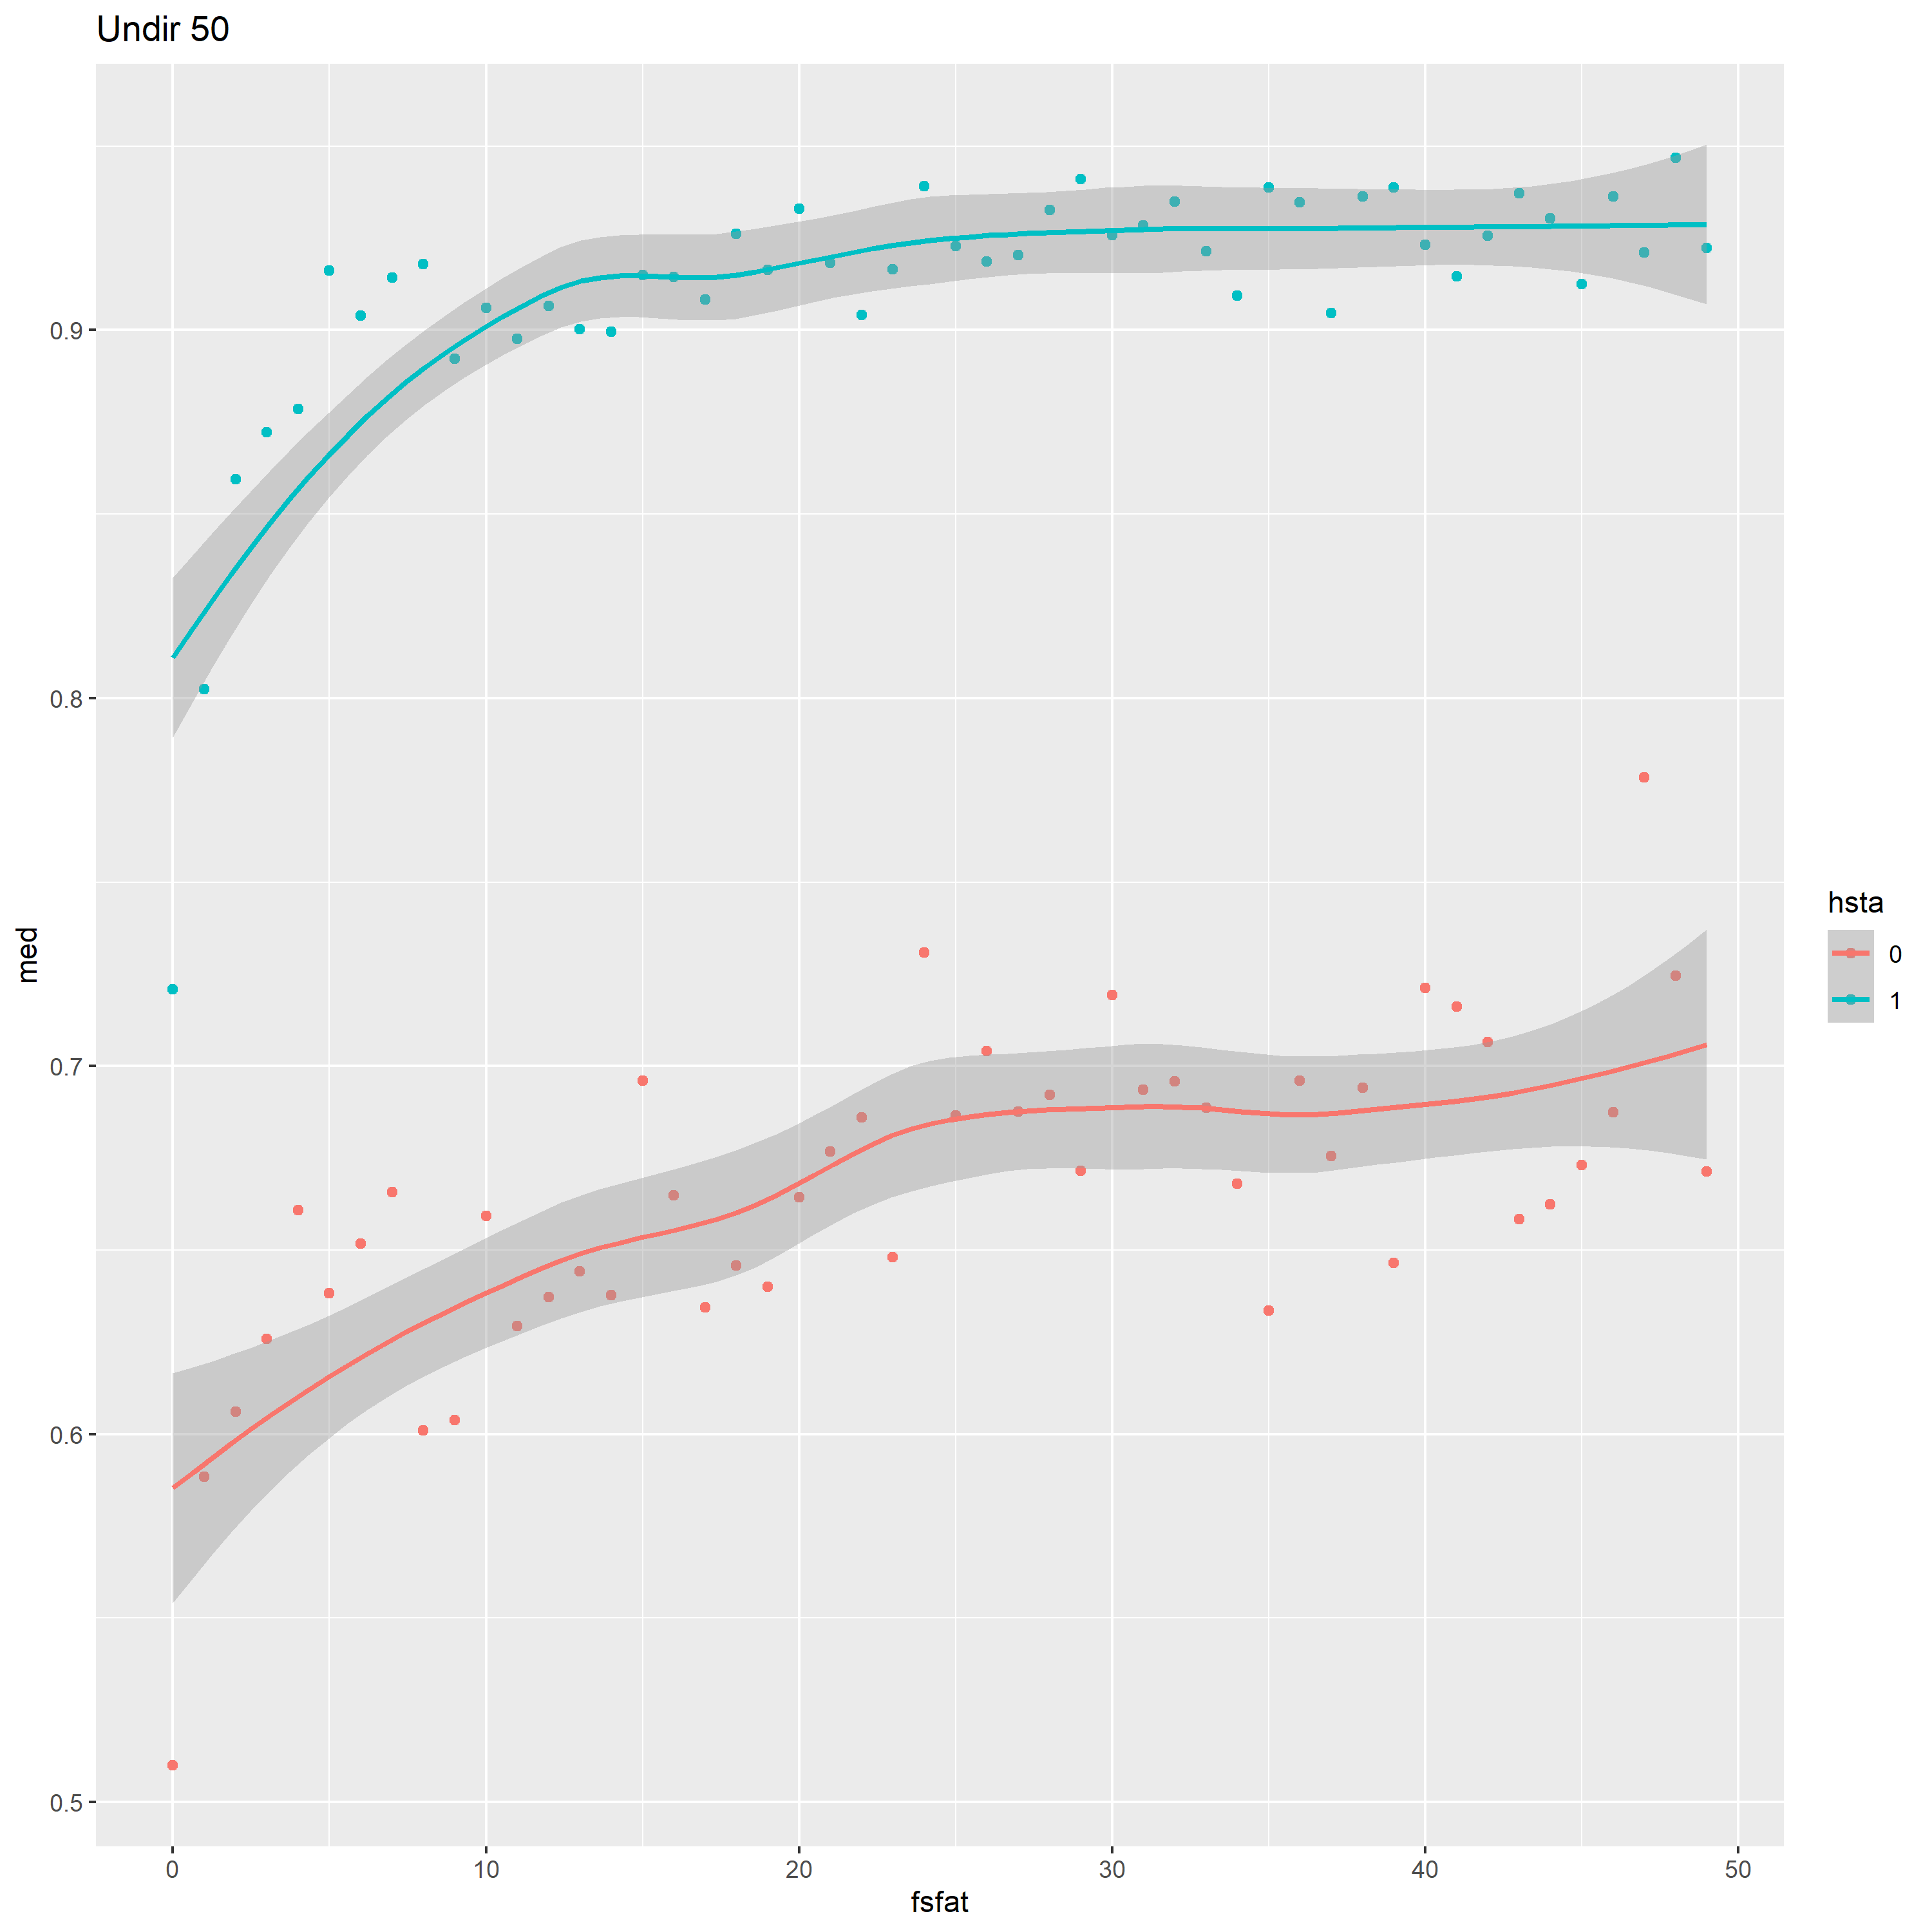
\includegraphics{Imgsimplify/plotbymean50.png}

Þar sést að það er einhver vöxtur í gangi hjá spurningum með nýjum svörum á meðan fleiri spurningum er svarað. En hvernig líta meðaltals línurnar út ef flokkað er með tilliti til hluta2 flokkana, skoðað bara fyrir tilvikin þegar hsta == 0?
Þá fæst svona mynd:
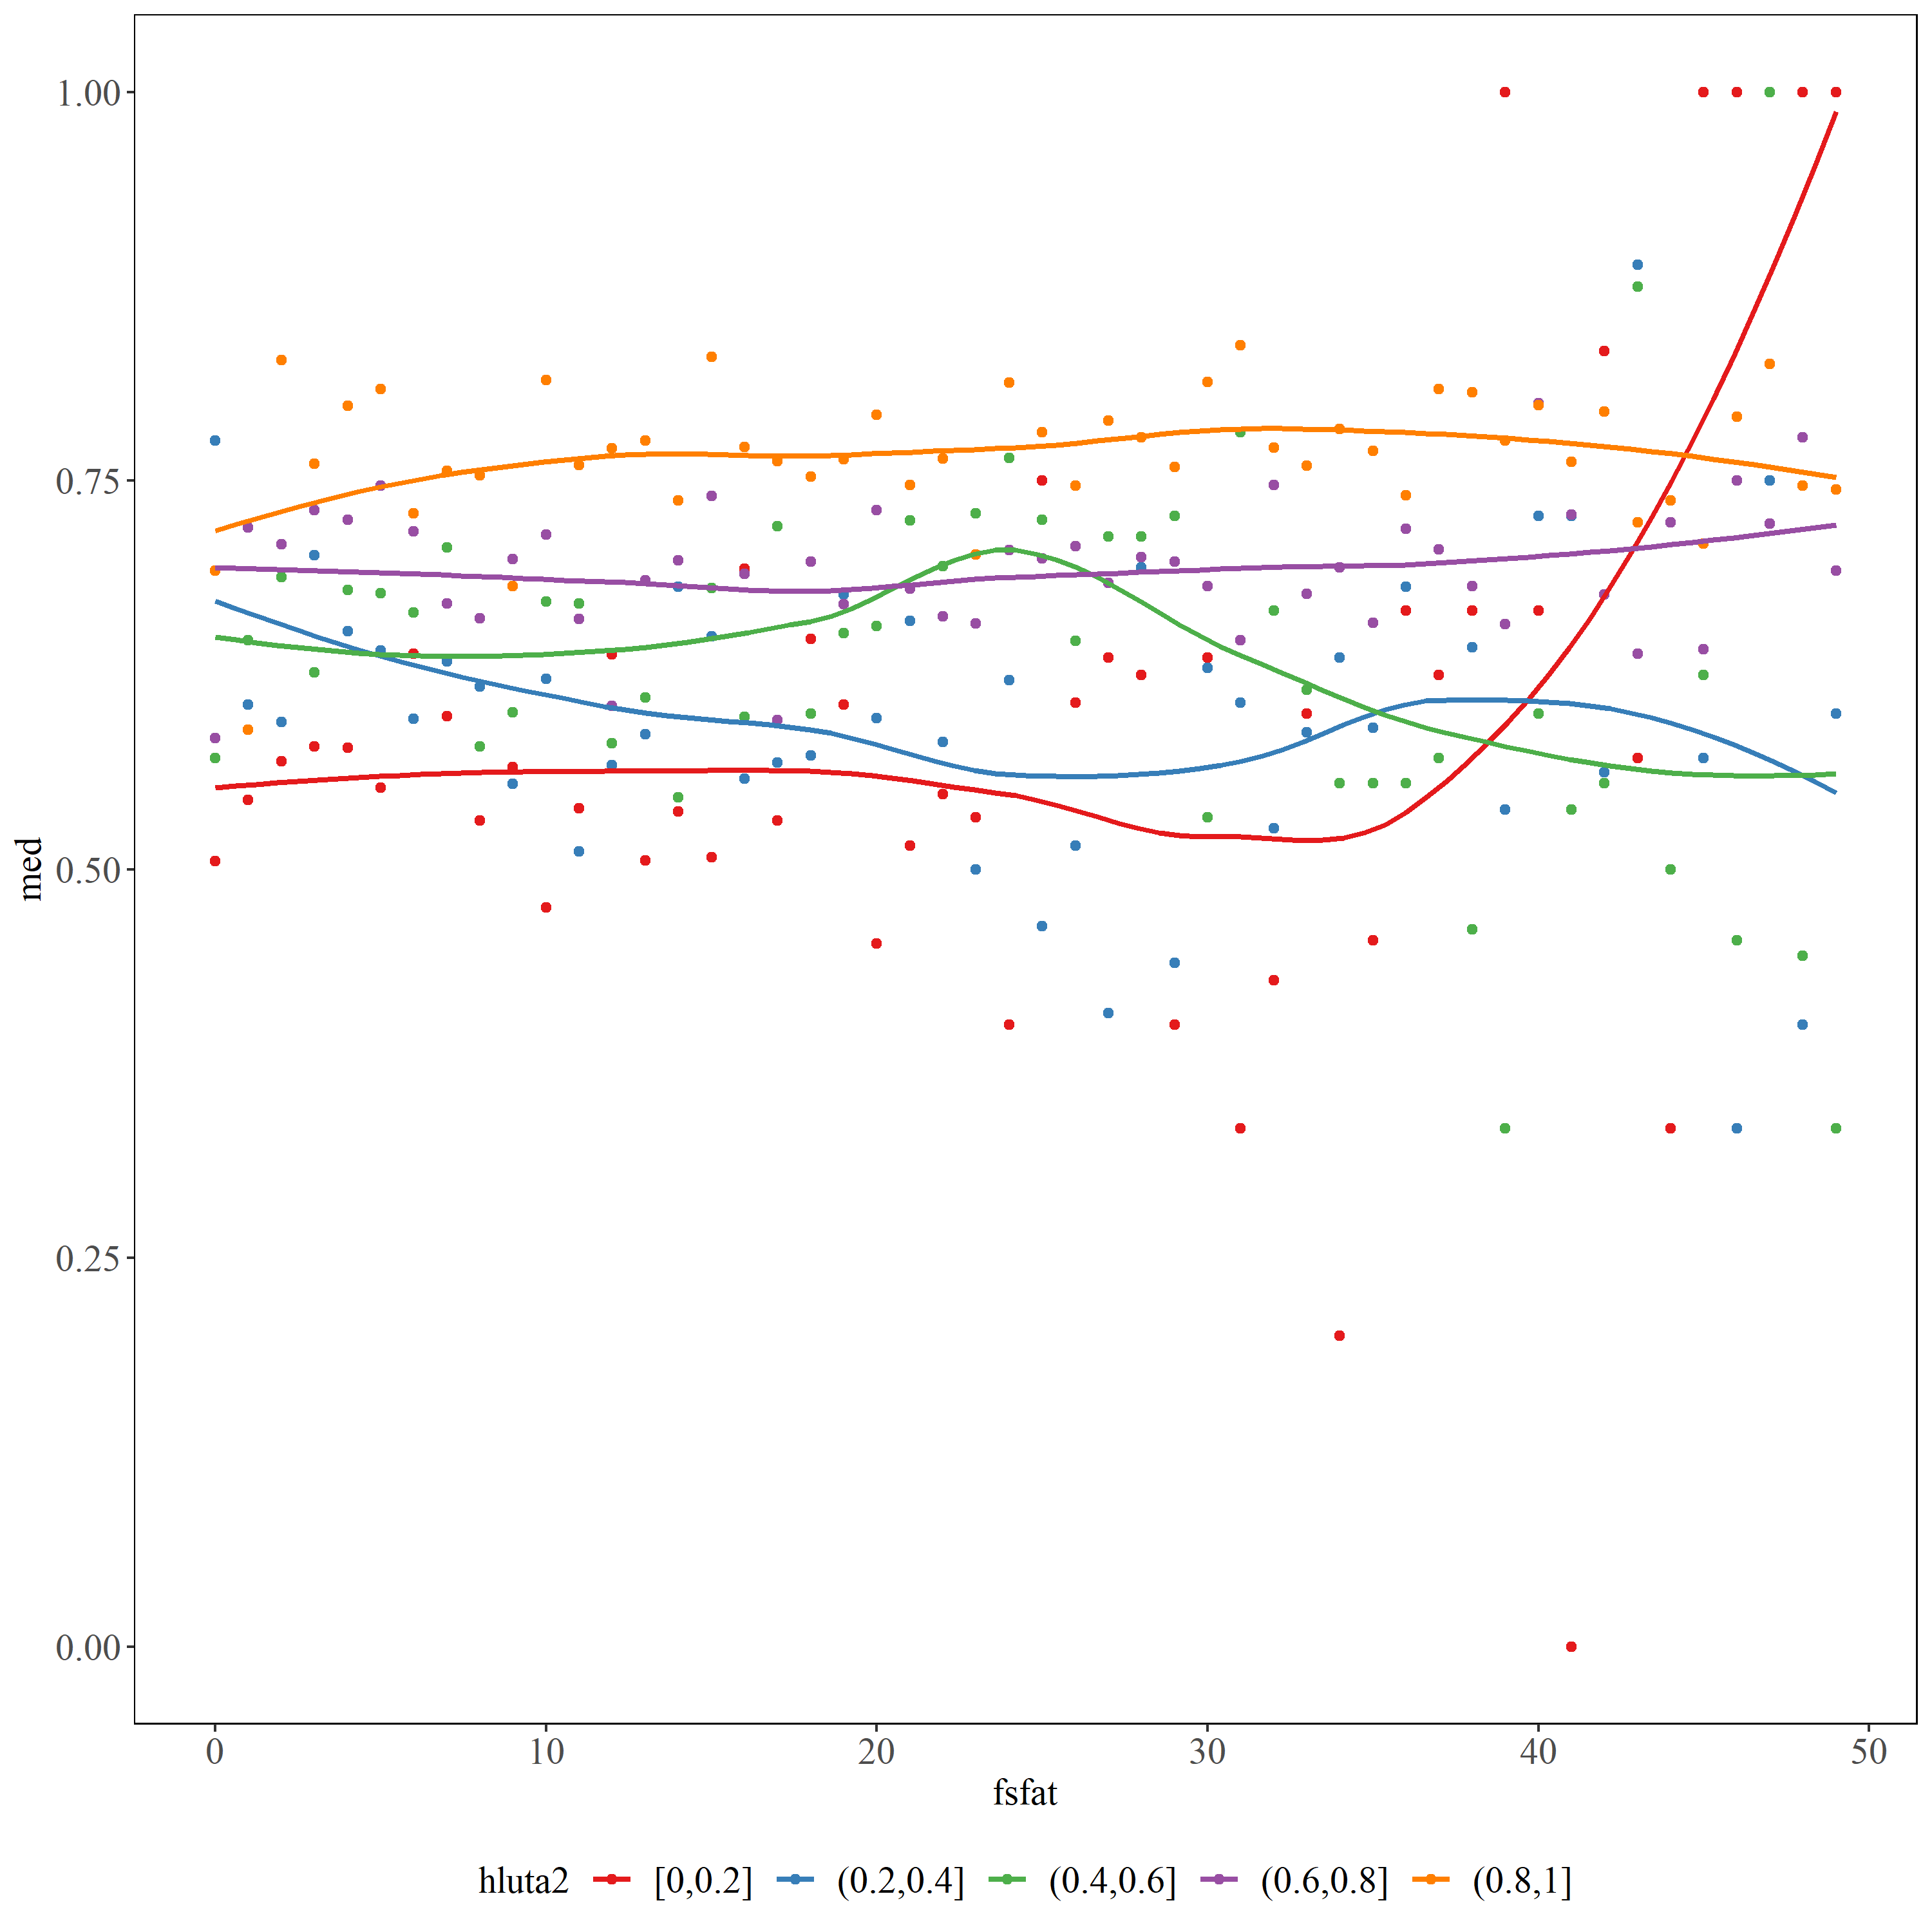
\includegraphics{Img/meanbyhlutfall.png}
Það er einhver stór vöxtur að koma hjá endanum, ég held að það kemur frá því að það eru ekki mikið af upplýsingum fyrir aftan suma punktana, svo ég teikna aftur upp myndina, nema að ég fjarlægji punkta þar sem ekki eru fleiri en 5 gildi fyrir aftan
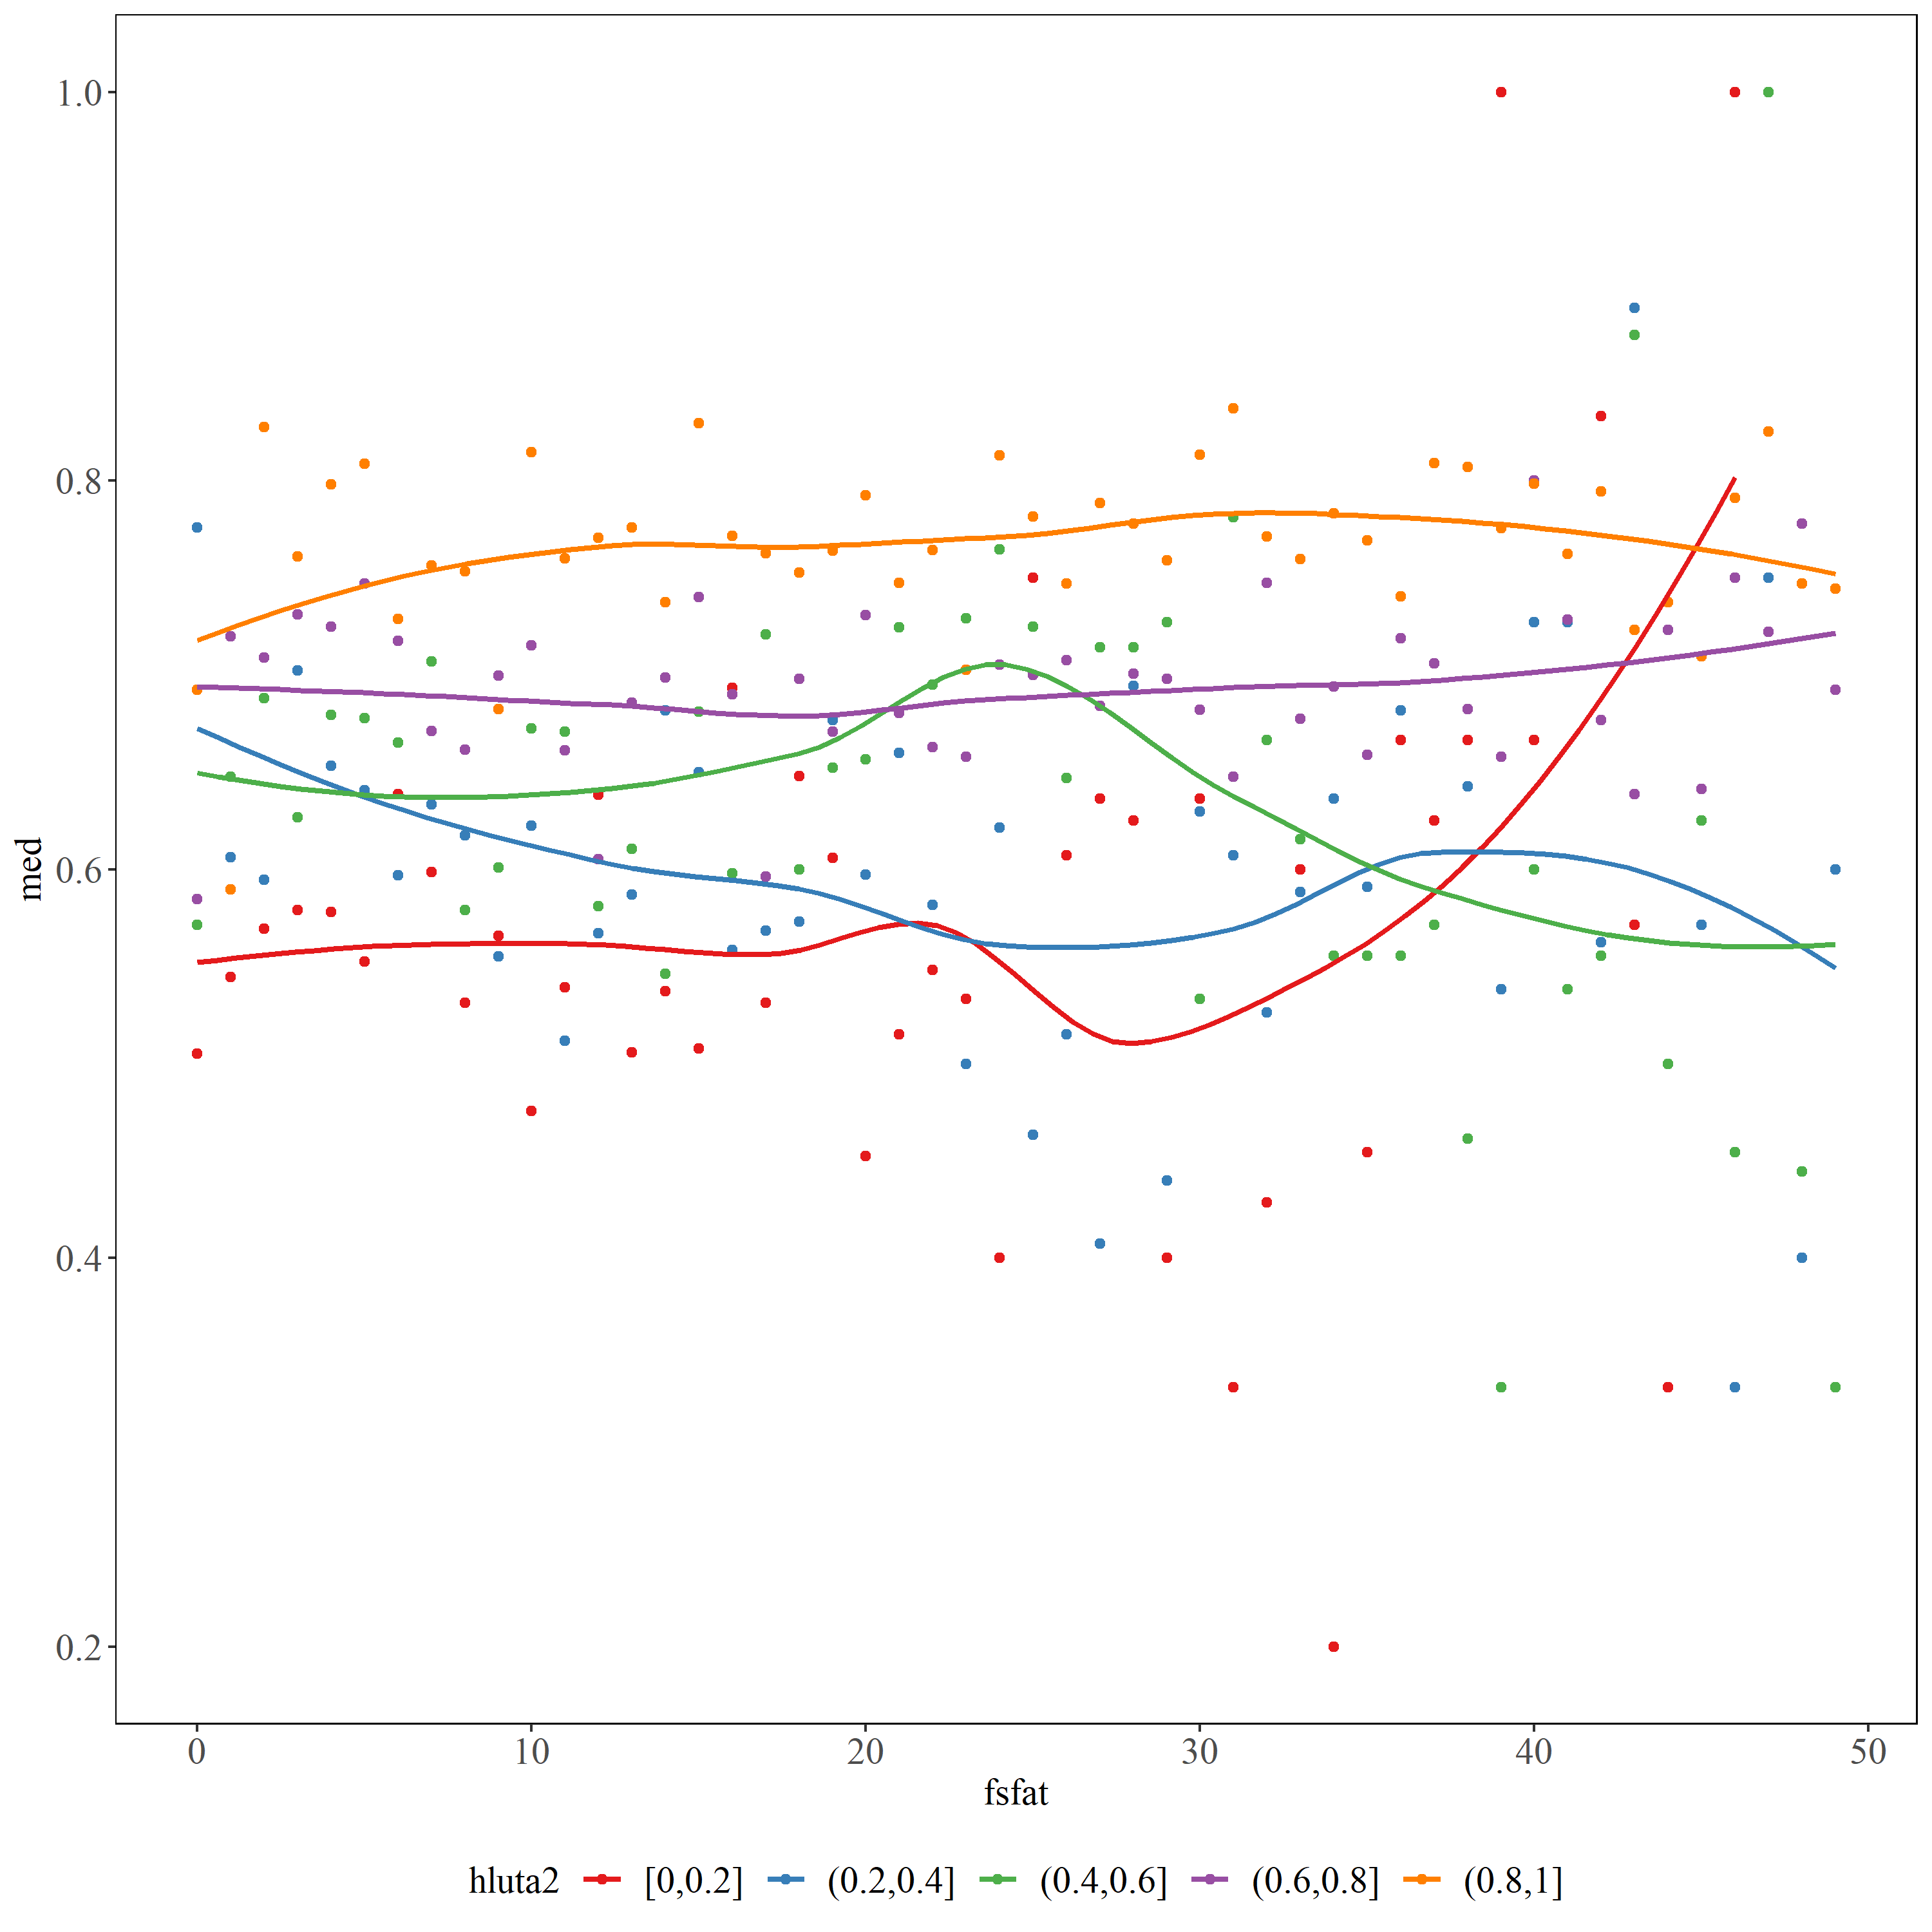
\includegraphics{Img/meanbyhlutfallLim.png}

Hér sést að línurnar eru aðeins beinar hér. Gott viðmið gæti komið ef prufað er að teikna línurnar ofan á upprunalegu meðaltals myndina
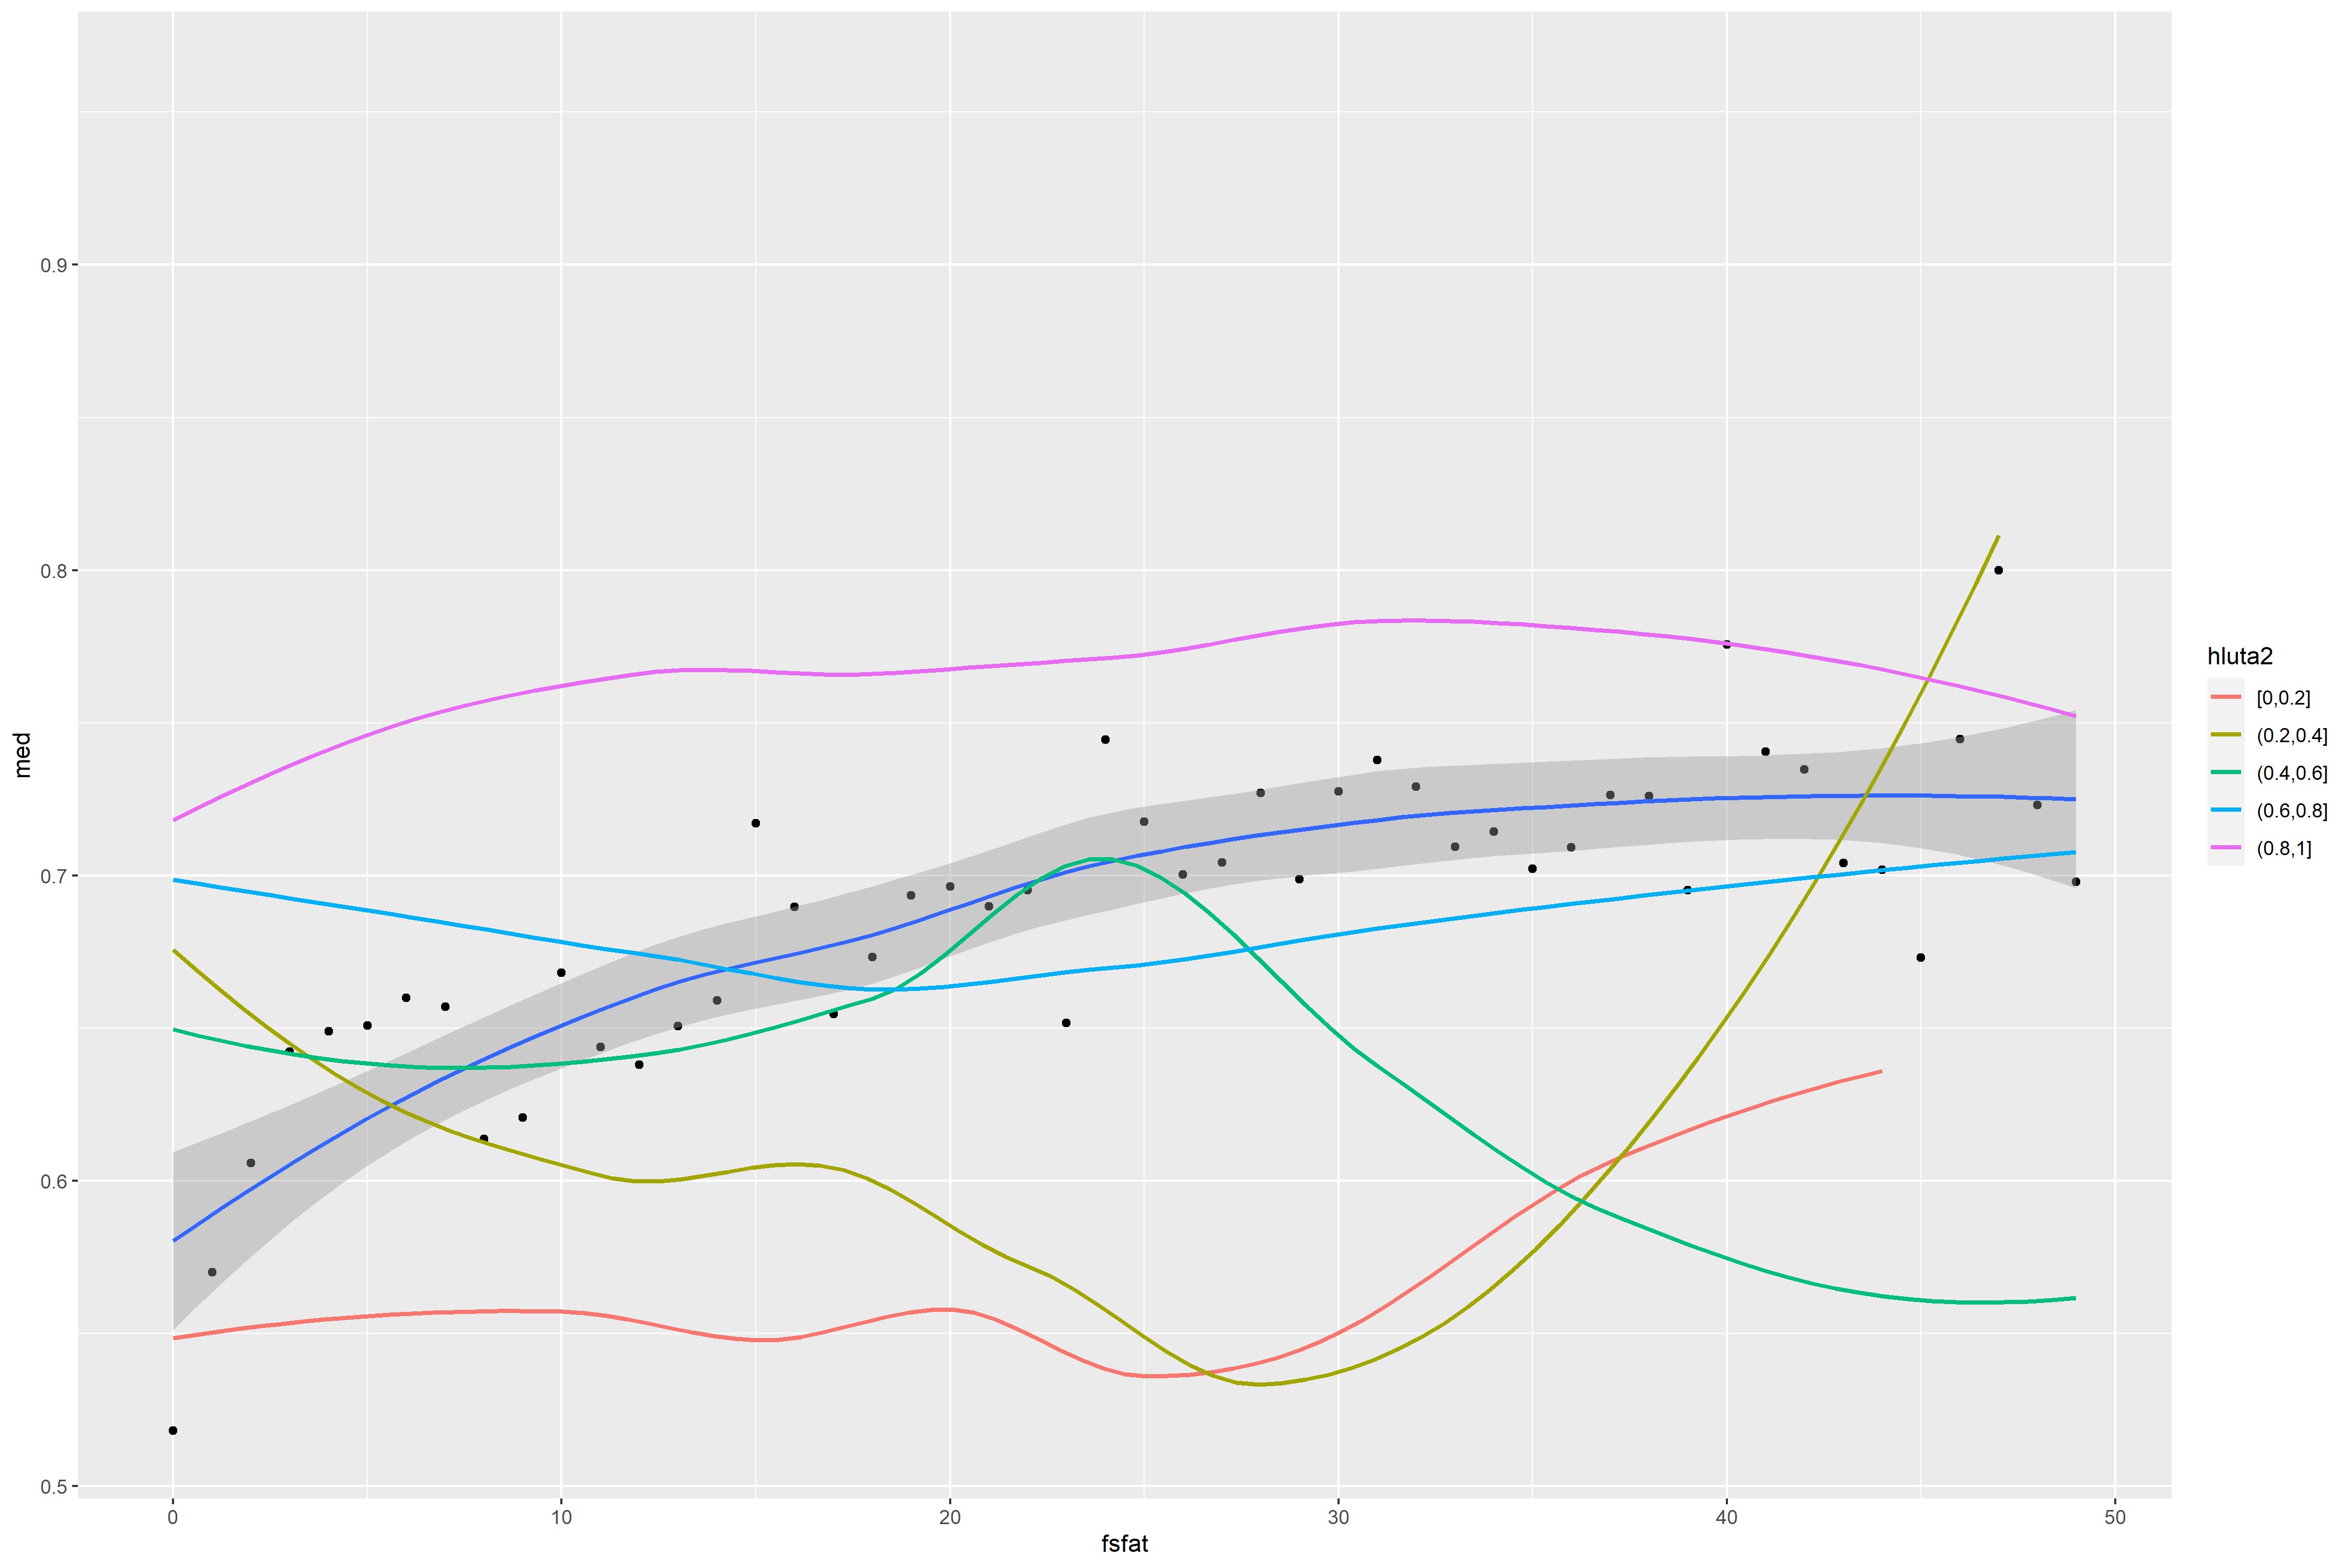
\includegraphics{Img/meabwhsbyhlutfall.png}
Þetta bentir til að fyrir aftan vöxtinn sem sást áðan, þá eru einhverjar hlutfalls breytur að toga að aftan.

\hypertarget{tuxf6flur}{%
\subsection{Töflur}\label{tuxf6flur}}

Gott er að skoða aðeins fjöldana fyrir aftan töfluna hér að ofan
T.d. er hægt að skoða hve mikið af gögnum það eru við hvert hlutfall

\begin{Shaded}
\begin{Highlighting}[]
\NormalTok{hashLim50 }\OperatorTok\StringTok{ }\KeywordTok{filter}\NormalTok{(hsta }\OperatorTok{==}\StringTok{ "0"}\NormalTok{) }\OperatorTok\StringTok{ }\KeywordTok{group_by}\NormalTok{(hluta2) }\OperatorTok
\StringTok{  }\KeywordTok{summarise}\NormalTok{(}\KeywordTok{n}\NormalTok{())}
\end{Highlighting}
\end{Shaded}

\begin{verbatim}
## # A tibble: 5 x 2
##   hluta2    `n()`
##   <fct>     <int>
## 1 [0,0.2]    8285
## 2 (0.2,0.4]  4667
## 3 (0.4,0.6]  3868
## 4 (0.6,0.8]  7028
## 5 (0.8,1]    7226
\end{verbatim}

\hypertarget{uppfuxe6ruxf0-model}{%
\subsection{uppfærð model}\label{uppfuxe6ruxf0-model}}

Þar sem komið er með nýja breytu, þá er hægt að skoða það miðað við upprunalega modelið og sjá hvernig það gengur
Keyri þrjú módel

\begin{Shaded}
\begin{Highlighting}[]
\NormalTok{fit1 <-}\StringTok{ }\KeywordTok{glmer}\NormalTok{(correct }\OperatorTok{~}\StringTok{ }\NormalTok{fsfat}\OperatorTok{*}\NormalTok{hsta }\OperatorTok{+}\StringTok{ }\NormalTok{nicc }\OperatorTok{+}\StringTok{ }\NormalTok{gpow }\OperatorTok{+}\StringTok{ }\NormalTok{lectureId }\OperatorTok{+}\StringTok{ }\NormalTok{(}\DecValTok{1} \OperatorTok{|}\StringTok{ }\NormalTok{studentId), }\DataTypeTok{family =} \KeywordTok{binomial}\NormalTok{(}\DataTypeTok{link =} \StringTok{"logit"}\NormalTok{), }
              \DataTypeTok{data =}\NormalTok{ hashLim100, }\DataTypeTok{nAGQ =} \DecValTok{0}\NormalTok{, }\DataTypeTok{control=}\KeywordTok{glmerControl}\NormalTok{(}\DataTypeTok{optimizer=}\StringTok{"bobyqa"}\NormalTok{,}\DataTypeTok{optCtrl=}\KeywordTok{list}\NormalTok{(}\DataTypeTok{maxfun=}\FloatTok{2e5}\NormalTok{)))}
\NormalTok{fit3 <-}\StringTok{ }\KeywordTok{glmer}\NormalTok{(correct }\OperatorTok{~}\StringTok{ }\NormalTok{hluta2}\OperatorTok{+}\NormalTok{hsta }\OperatorTok{+}\StringTok{ }\NormalTok{nicc }\OperatorTok{+}\StringTok{ }\NormalTok{gpow }\OperatorTok{+}\StringTok{ }\NormalTok{lectureId }\OperatorTok{+}\StringTok{ }\NormalTok{(}\DecValTok{1} \OperatorTok{|}\StringTok{ }\NormalTok{studentId), }\DataTypeTok{family =} \KeywordTok{binomial}\NormalTok{(}\DataTypeTok{link =} \StringTok{"logit"}\NormalTok{), }
              \DataTypeTok{data =}\NormalTok{ hashLim100, }\DataTypeTok{nAGQ =} \DecValTok{0}\NormalTok{, }\DataTypeTok{control=}\KeywordTok{glmerControl}\NormalTok{(}\DataTypeTok{optimizer=}\StringTok{"bobyqa"}\NormalTok{,}\DataTypeTok{optCtrl=}\KeywordTok{list}\NormalTok{(}\DataTypeTok{maxfun=}\FloatTok{2e5}\NormalTok{)))}
\NormalTok{fit7 <-}\StringTok{ }\KeywordTok{glmer}\NormalTok{(correct }\OperatorTok{~}\StringTok{ }\NormalTok{hluta2 }\OperatorTok{+}\StringTok{ }\NormalTok{fsfat }\OperatorTok{+}\StringTok{ }\NormalTok{hsta }\OperatorTok{+}\StringTok{ }\NormalTok{nicc }\OperatorTok{+}\StringTok{ }\NormalTok{gpow }\OperatorTok{+}\StringTok{ }\NormalTok{lectureId }\OperatorTok{+}\StringTok{ }\NormalTok{(}\DecValTok{1} \OperatorTok{|}\StringTok{ }\NormalTok{studentId), }\DataTypeTok{family =} \KeywordTok{binomial}\NormalTok{(}\DataTypeTok{link =} \StringTok{"logit"}\NormalTok{), }
              \DataTypeTok{data =}\NormalTok{ hashLim100, }\DataTypeTok{nAGQ =} \DecValTok{0}\NormalTok{, }\DataTypeTok{control=}\KeywordTok{glmerControl}\NormalTok{(}\DataTypeTok{optimizer=}\StringTok{"bobyqa"}\NormalTok{,}\DataTypeTok{optCtrl=}\KeywordTok{list}\NormalTok{(}\DataTypeTok{maxfun=}\FloatTok{2e5}\NormalTok{)))}
\end{Highlighting}
\end{Shaded}

Hér er:
* fit1: upprunalega líkanið

\begin{itemize}
\item
  fit3: upprunalega líkanið, nema það er víxlað fsfat fyrir hluta2
\item
  fit7: það er líkan sem hefur bæði fsfat og hluta2
\end{itemize}

Gott er kannski að skoða muninn á milli þeirra, með anova

\begin{Shaded}
\begin{Highlighting}[]
\KeywordTok{anova}\NormalTok{(fit1, fit3)}
\end{Highlighting}
\end{Shaded}

\begin{verbatim}
## Data: hashLim100
## Models:
## fit1: correct ~ fsfat * hsta + nicc + gpow + lectureId + (1 | studentId)
## fit3: correct ~ hluta2 + hsta + nicc + gpow + lectureId + (1 | studentId)
##      npar   AIC   BIC logLik deviance Chisq Df Pr(>Chisq)    
## fit1   24 62028 62253 -30990    61980                        
## fit3   26 61571 61815 -30760    61519   461  2  < 2.2e-16 ***
## ---
## Signif. codes:  0 '***' 0.001 '**' 0.01 '*' 0.05 '.' 0.1 ' ' 1
\end{verbatim}

\begin{Shaded}
\begin{Highlighting}[]
\KeywordTok{anova}\NormalTok{(fit3, fit7)}
\end{Highlighting}
\end{Shaded}

\begin{verbatim}
## Data: hashLim100
## Models:
## fit3: correct ~ hluta2 + hsta + nicc + gpow + lectureId + (1 | studentId)
## fit7: correct ~ hluta2 + fsfat + hsta + nicc + gpow + lectureId + (1 | 
## fit7:     studentId)
##      npar   AIC   BIC logLik deviance  Chisq Df Pr(>Chisq)    
## fit3   26 61571 61815 -30760    61519                         
## fit7   27 61178 61431 -30562    61124 395.34  1  < 2.2e-16 ***
## ---
## Signif. codes:  0 '***' 0.001 '**' 0.01 '*' 0.05 '.' 0.1 ' ' 1
\end{verbatim}

Hér segjir að fit3 er marktækara en fit1 og fit7 er marktækara en fit3.
Gott er að skoða aðeins standardized brier score muninn hjá þeim og svo líka AUC muninn

\begin{Shaded}
\begin{Highlighting}[]
\NormalTok{sb1 <-}\StringTok{ }\KeywordTok{SBrierScore}\NormalTok{(fit1, hashLim100)}
\NormalTok{sb3 <-}\StringTok{ }\KeywordTok{SBrierScore}\NormalTok{(fit3, hashLim100)}
\NormalTok{sb7 <-}\StringTok{ }\KeywordTok{SBrierScore}\NormalTok{(fit7, hashLim100)}

\NormalTok{fitauc1 <-}\StringTok{ }\KeywordTok{AUC}\NormalTok{(}\KeywordTok{predict}\NormalTok{(fit1, }\DataTypeTok{type =} \StringTok{"response"}\NormalTok{), hashLim100}\OperatorTok{$}\NormalTok{correct)}
\NormalTok{fitauc3 <-}\StringTok{ }\KeywordTok{AUC}\NormalTok{(}\KeywordTok{predict}\NormalTok{(fit3, }\DataTypeTok{type =} \StringTok{"response"}\NormalTok{), hashLim100}\OperatorTok{$}\NormalTok{correct)}
\NormalTok{fitauc7 <-}\KeywordTok{AUC}\NormalTok{(}\KeywordTok{predict}\NormalTok{(fit7, }\DataTypeTok{type =} \StringTok{"response"}\NormalTok{), hashLim100}\OperatorTok{$}\NormalTok{correct)}

\NormalTok{sb1}
\end{Highlighting}
\end{Shaded}

\begin{verbatim}
## [1] 0.2411666
\end{verbatim}

\begin{Shaded}
\begin{Highlighting}[]
\NormalTok{sb3}
\end{Highlighting}
\end{Shaded}

\begin{verbatim}
## [1] 0.2479733
\end{verbatim}

\begin{Shaded}
\begin{Highlighting}[]
\NormalTok{sb7}
\end{Highlighting}
\end{Shaded}

\begin{verbatim}
## [1] 0.2524708
\end{verbatim}

\begin{Shaded}
\begin{Highlighting}[]
\NormalTok{fitauc1}
\end{Highlighting}
\end{Shaded}

\begin{verbatim}
## [1] 0.8331737
\end{verbatim}

\begin{Shaded}
\begin{Highlighting}[]
\NormalTok{fitauc3}
\end{Highlighting}
\end{Shaded}

\begin{verbatim}
## [1] 0.8358489
\end{verbatim}

\begin{Shaded}
\begin{Highlighting}[]
\NormalTok{fitauc7}
\end{Highlighting}
\end{Shaded}

\begin{verbatim}
## [1] 0.8392987
\end{verbatim}

Það er smár munur milli hverja, en ekki það mikill. Munurinn hjá standardized brier fyrir fit1 og fit3 er bara 0.0068. Sem segir til að munurinn á að nota hlutfall rangra svara séð í staðinn fyrir fjöldi spurninga fram að þessu er mjög lítill miðað við standardized brier. Það gæti verið að benda til að það gæti verið að áhrifinn að aftan vöxtinn hjá fsfat er aðallega bara hluta2.
Að sama dúr er líka bara aðeins betra milli fit3 og fit7, með 0.0045, sem er enn minni en hinn. Svo á meðan það er marktækur munur á milli fit3 og fit7, þá er fit7 ekki endilega það mikið betra en fit3.
Sömu niðurstöðurnar ef skoðað er munin hjá AUC í fit1 og fit3 0.0027 og munin milli fit3 og fit7 sem 0.0034. Á meðan AUC vex smá, þá er það ekki endilega nógu mikið til að segja til hvort eitt er betra en hitt. Ef ég skil þetta rétt.

\hypertarget{teikna-fyrir-model}{%
\subsection{Teikna fyrir model}\label{teikna-fyrir-model}}

Svo í lokinn, er kannski gott að geta teiknað upp fyrir hvert þeirra predicted effect á móti correct, til að sjá hvernig það lítur út
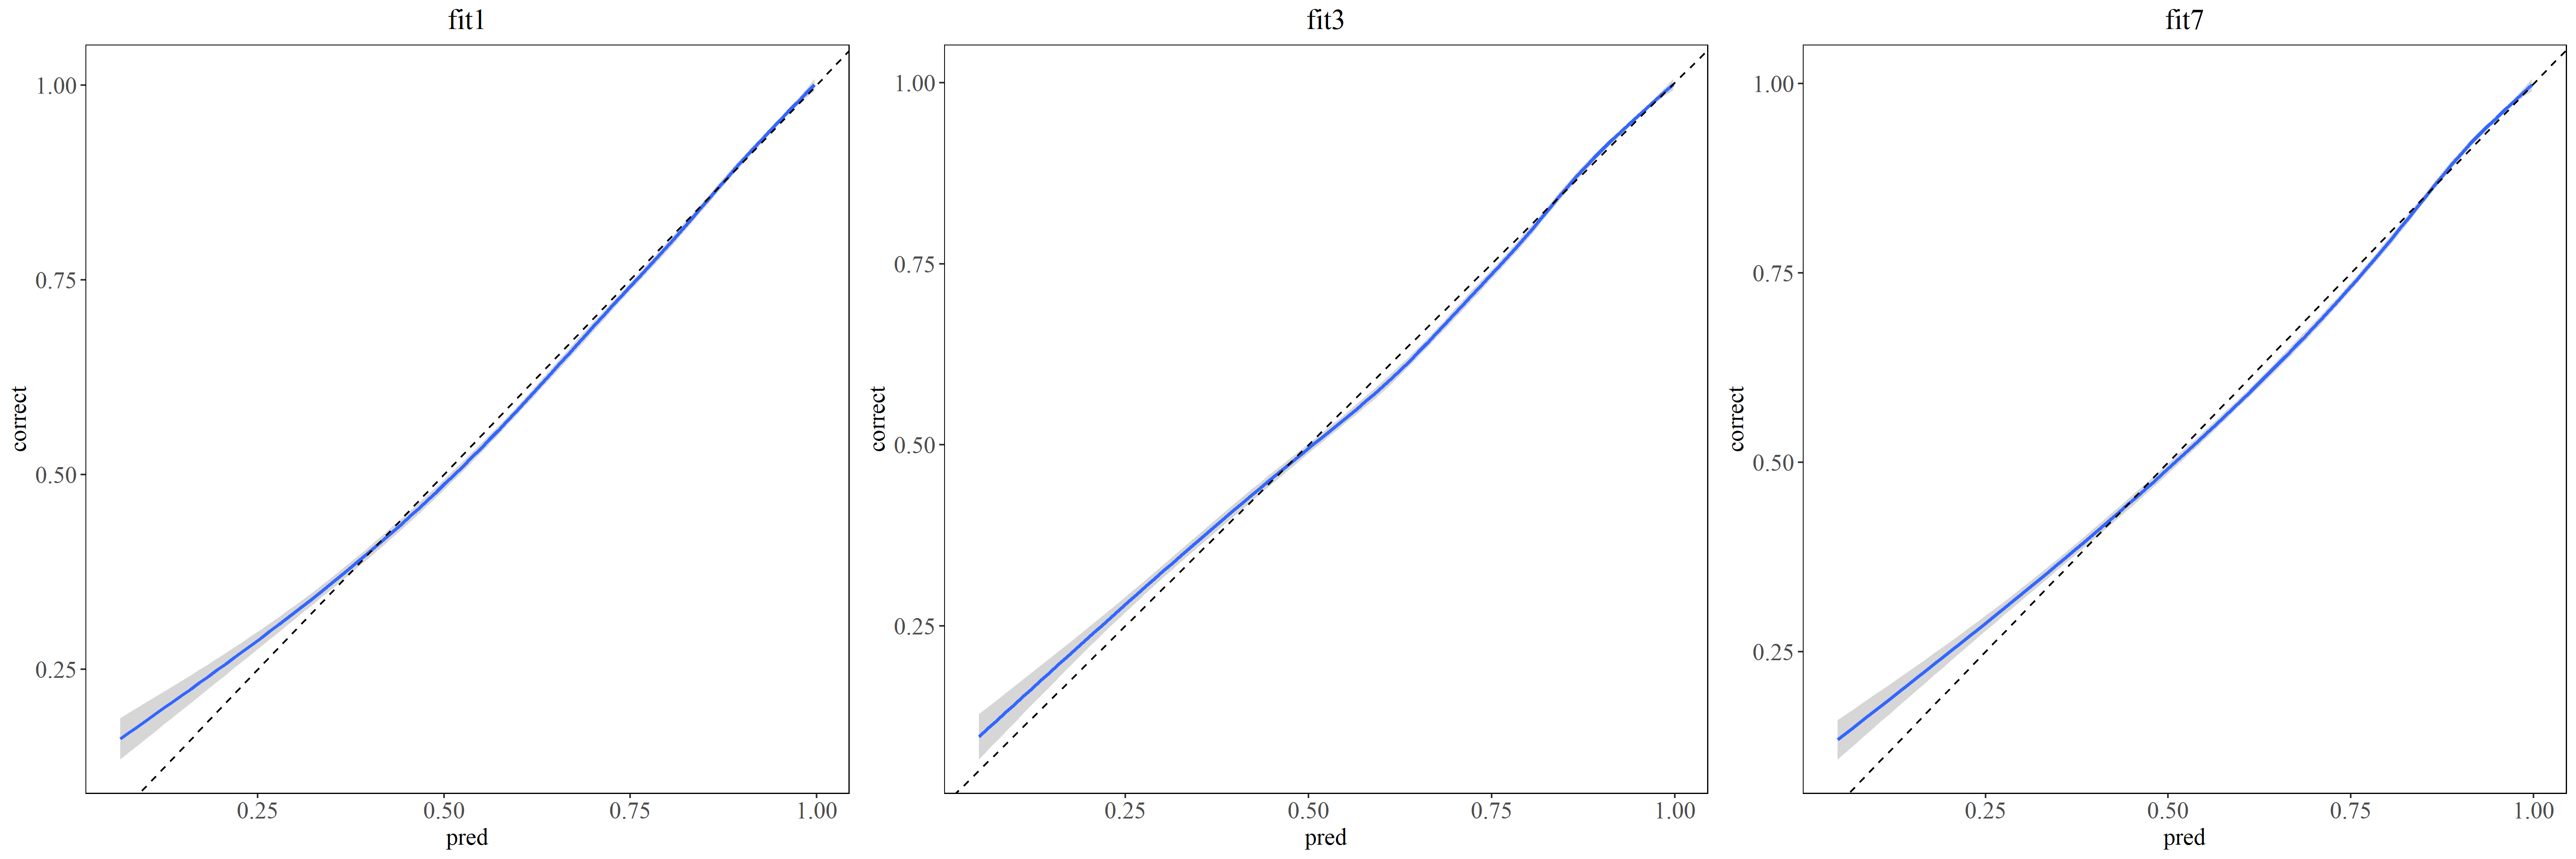
\includegraphics{Img/predplot.png}

Það lítur út fyrir að vera beint að mesta lagi, sem bendir að það er að ná vel á móti alvöru niðurstöðunum. En það er ekki mikill munur á milli þeirra. Svo eitt er ekki endilega betra en næsta?

\end{document}
